%\documentclass[12pt]{report}
\documentclass[utf8, 14pt]{G7-32}  % ГОСТ 7.32-2001
%----------------------------------------------------------
% Значения констант по КП, НИРС, ВКР
%----------------------------------------%
% общие определения
\newcommand{\UpperFullOrganisationName}{Министерство науки и высшего образования Российской Федерации}
\newcommand{\ShortOrganisationName}{МГТУ~им.~Н.Э.~Баумана}
\newcommand{\FullOrganisationName}{федеральное государственное бюджетное образовательное\newline учреждение высшего профессионального образования\newline <<Московский государственный технический университет имени Н.Э.~Баумана\newline (национальный исследовательский университет)>> (\ShortOrganisationName)}
\newcommand{\OrganisationAddress}{105005, Россия, Москва, ул.~2-ая Бауманская, д.~5, стр.~1}
%----------------------------------------%
\newcommand{\gitlabdomain}{sa2systems.ru:88}
%----------------------------------------------------------
\newcommand{\doctypesid}{kp} % vkr (выпускная квалификационная работа) / kp (курсовой проект) / kr (курсовая работа) / nirs (научно-исследовательская работа студента) / nkr (научно-квалификационная работа)

% Тема должна быть сформулирована так, чтобы рассказать, о чем работа, но сделать это так, чтобы у читателя возникло желание читать аннота-цию. При формулировке темы не следует стараться рассказать о работе всё. Пример корректной темы: "Математическое моделирование процесса размножения медуз в Южно-Китайском море". Пример некорректной темы: "Применение модели SIS для моделирования процесса размножения медуз в Южно-Китайском море с использованием метода Рунге-Кутты и многопроцессорных вычислительных систем".
\newcommand{\Title}{Разработка механизма вывода типов с использованием системы типов Хиндли-Милнера}%{}
\newcommand{\TitleSource}{кафедра} % кафедра, предприятие, НИР, НИР кафедры, заказ организации

\newcommand{\SubTitle}{по дисциплине <<Модели и методы анализа проектных решений>>} % Методы оптимизации
\newcommand{\faculty}{<<Робототехника и комплексная автоматизация>>}
\newcommand{\facultyShort}{РК}
\newcommand{\department}{<<Системы автоматизированного проектирования (РК-6)>>}
\newcommand{\departmentShort}{РК-6}

\newcommand{\Author}{Никитин В.Л.}
\newcommand{\AuthorFull}{Никитин Владимир Леонидович}
\newcommand{\ScientificAdviserPosition}{доктор физико-математических наук}    % Должность научного руководителя
\newcommand{\ScientificAdviser}{Соколов А.П.}    % Научный руководитель
\newcommand{\ConsultantA}{Соколов А.П.}                % Консультант 1
% \newcommand{\ConsultantB}{@Фамилия~И.О.@}				% Консультант 2
\newcommand{\Normocontroller}{Грошев~С.В.}        % Нормоконтролёр
\newcommand{\group}{РК6-75Б}
\newcommand{\Semestr}{осенний семестр} % Например: осенний семестр или весенний семестр
\newcommand{\BeginYear}{2023}
\newcommand{\Year}{2024}
\newcommand{\Country}{Россия}
\newcommand{\City}{Москва}
\newcommand{\TaskStatementDate}{<<\underline{\textit{01}}>> \underline{октября} \Year~г.} %Дата выдачи задания

\newcommand{\depHeadPosition}{Заведующий кафедрой}        % Должность руководителя подразделения
\newcommand{\depHeadName}{А.П.~Карпенко}        % Должность руководителя подразделения

% Цель выполнения 
\newcommand{\GoalOfResearch}{реализация системы вывода и проверки типов} % с маленькой буквы и без точки на конце

% Объектом исследования называют то, что исследуется в работе. Например, для указанной выше темы объектом может быть популяция медуз, но никак ни модель SIS, ни Южно-Китайское море, ни метод моделирования популяции медуз. 
\newcommand{\ObjectOfResearch}{система типов}

% Предмет исследований (уже чем объект, определяется, исходя из задач: формулируется как существительное, как правило, во множественном числе, определяющее "конкретный объект исследований" среди прочих в рамках более общего)
\newcommand{\SubjectOfResearch}{система типов Хиндли-Милнера}

% Основная задача, на решение которой направлена работа
\newcommand{\MainProblemOfResearch}{реализация алгоритма вывода типов на основе выбранной системы типов}

% Выполненные задачи
\newcommand{\SubtasksPerformed}{%
    В результате выполнения работы:
    \begin{inparaenum}[1)]
        \item спроектировано представление абстрактного синтаксического дерева в компиляторе;
        \item реализован семантический анализатор;
        \item показано, что компилятор успешно может вывести тип функции
    \end{inparaenum}}

% Ключевые слова (представляются для обеспечения потенциальной возможности индексации документа)
\newcommand{\keywordsru}{%
    теория типов, языки программирования, компиляторы, фукнциональное программирование, система типов Хиндли-Милнера} % 5-15 слов или выражений на русском языке, для разделения СЛЕДУЕТ ИСПОЛЬЗОВАТЬ ЗАПЯТЫЕ
\newcommand{\keywordsen}{%
    type theory, programming languages, compilers, functional programming, Hindley-Milner type system} % 5-15 слов или выражений на английском языке, для разделения СЛЕДУЕТ ИСПОЛЬЗОВАТЬ ЗАПЯТЫЕ

% Краткая аннотация
\newcommand{\Preface}{
	Работа посвящена реализации механизма вывода типов для языка программирования Kodept.
	Программирование выстроено вокруг глубокой математической теории.
	Благодаря этому появляются возможности для оптимизации, развития и улучшения языков посредством применения математики.
	Одним из важных применений является теория типов, которая помогает программисту в написании кода.
	В последнее время все больше и больше языков почерпывают что-то из этой области.
	Применение мощной системы типов позволяет зачастую снизить количество ошибок, возникающих при разработке.
} % с большой буквы с точкой в конце

%----------------------------------------%
% выходные данные по документу
\newcommand{\DocOutReference}{\Author. \Title\xspace\SubTitle. [Электронный ресурс] --- \City: \Year. --- \total{page} с. URL:~\url{https://\gitlabdomain} (система контроля версий кафедры РК6)}

%----------------------------------------------------------


%----------------------------------------------------------
%общая преамбула для всех лабораторных - настройки общего вида оформления
%----------------------------------------------------------
\usepackage{amsfonts}
\usepackage{amsmath}
%\usepackage{mathabx}
%----------------------------------------------------------
\newcommand{\doclicense}{\includegraphics[width=0.09\textwidth]{doc-spec/by.eps}\xspace}%\ccShareAlike

\usepackage[T2A]{fontenc}
\usepackage[utf8]{inputenc}
\usepackage[russian]{babel} %% это необходимо для включения переносов english
\usepackage{float}
\usepackage{rotating}
\usepackage{multirow}
\usepackage{pdflscape}
\usepackage{bm}
% необходимо для возможности копирования и поиска в готовом PDF
%\usepackage{cmap} 
\usepackage{array}
\usepackage{multicol}
\usepackage{relsize}
\usepackage{booktabs}
% Пакет необходим для поддержки многострочного подчеркивания текста
\usepackage[normalem]{ulem}

%----------------------------------------------------------------
% Сохранение метаданных в PDF об авторе документа
\usepackage{hyperxmp}
\usepackage{hyperref}
\hypersetup{%
    bookmarks=false,        % show bookmarks bar?
    pdftoolbar=true,        % show Acrobat’s toolbar?
    pdfmenubar=true,        % show Acrobat’s menu?
    pdffitwindow=false,     % window fit to page when opened
    pdfstartview={FitH},    % fits the width of the page to the window
    pdftitle={\Title},    	% title
    pdfauthor={\Author},    % author
%		pdfcopyright={Copyright © \Year, \Author. Все права защищены.},
		pdfcopyright={CC BY 4.0, \Year, \Author.},
		pdflicenseurl={http://creativecommons.org/licenses/by/4.0/},
    pdfsubject={\SubjectOfResearch},   % subject of the document
    pdfcreator={\pdftexbanner},   % creator of the document
%		pdfpublisher={Computer-aided design department, Bauman Moscow State Technical University},
		pdfcaptionwriter={Ass. Prof., PhD. Alexandr P. Sokolov},
    pdfproducer={\Author, \group, \Year, Computer-aided design department, Bauman Moscow State Technical University}, % producer of the document
    pdfkeywords={\keywordsru, \keywordsen}, % producer of the document
    pdfnewwindow=true,      % links in new window
    colorlinks=true,
    citecolor=purple,
    linkcolor=red,      % color of internal links (change box color with linkbordercolor)
    urlcolor=green,
    filecolor=black      % color of file links
}
%----------------------------------------------------------------
\usepackage{xspace}
%----------------------------------------------------------
\usepackage[style=long4colheader, translate=babel, section=chapter, toc]{glossaries}
\usepackage[abbreviations, toc=true, xindy, automake]{glossaries-extra}
\setglossarystyle{treenoname}%+
\makeglossaries
%----------------------------------------------------------
% поддержка inparaenum
\usepackage{paralist} 
%----------------------------------------------------------
% нужно для определения окружения description
%\usepackage{enumitem} 
%----------------------------------------------------------------
% Настройки вставки PDF (для вставки, к примеру, направления на защиту, акта об отсутствии заимствования, рецензии)
\usepackage{pdfpages}
\includepdfset{turn=true,scale=0.95,pages=-,pagecommand={\pagestyle{fancy}}}
%----------------------------------------------------------
\usepackage{tikz}
\usetikzlibrary{tikzmark}
\usetikzlibrary{matrix,automata,graphs}
\usetikzlibrary{arrows,positioning,trees}
%----------------------------------------------------------
% необходимо для возможности включать в имена включаемых файлов _
\usepackage[strings]{underscore}
%----------------------------------------------------------
% добавление поддержки команды вывода текста на полях \marginnote
\usepackage{marginnote}
% добавление поддержки команды \color
\usepackage{xcolor}
%--------------------------------------------
% final - удаляет все всплывающие комментарии
\usepackage[author={Alexandr Sokolov},opacity=0.1]{pdfcomment}
%\usepackage[author={Alexandr Sokolov},opacity=0.1,final]{pdfcomment}
\newcommand{\messnote}[1]{\marginnote{\color[rgb]{1,0,0}\Huge\textbf{!}\pdfcomment{#1}}[-1.0cm]}
%----------------------------------------------------------
% Произвольная нумерация списков.
\usepackage{enumerate}
%----------------------------------------------------------
%\raggedbottom
%\textwidth=163mm
%\textheight=220mm
%\oddsidemargin=-0.5pt
%\footskip=30pt
%\topmargin=27pt
%\headheight=12pt
%\headsep=25pt
%\topskip=10pt
%\baselineskip=15pt
%\topmargin=-4mm
%----------------------------------------------------------
\tolerance 1414
\hbadness 1414
\emergencystretch 1.5em
\hfuzz 0.3pt
\widowpenalty=10000
\vfuzz \hfuzz
\raggedbottom
%----------------------------------------------------------
% Настройки колонтитулов
\usepackage{fancyhdr} % Headers and footers
\fancyhf{} % clear all headers and footers - equivalent to %\fancyhead{} and \fancyfoot{}
\renewcommand{\headrulewidth}{0.0pt}
\renewcommand{\footrulewidth}{0.0pt}
\renewcommand{\chaptermark}[1]{\markboth{ \chaptername\ \thechapter }{}} 
%\renewcommand{\chaptermark}[1]{\markboth{ \chaptername\ \thechapter ~ \ #1}{}} 
%\renewcommand{\sectionmark}[1]{\markright{\thesection ~ \ #1}}

%head setting
\fancyhead[C]{\thepage}
\fancyfoot[C]{}
\setlength{\headheight}{17pt}%

\pagestyle{fancy} % All pages have headers and footers
%----------------------------------------%
%Необходимо для того, чтобы при использовании команды \thispagestyle{plain} стиль plain был переопределён на этот
\fancypagestyle{plain}{%
\fancyhf{}% clear all header and footer fields
\renewcommand{\headrulewidth}{0pt}%
\renewcommand{\footrulewidth}{0pt}%
\fancyhead[C]{\thepage}
\fancyfoot[C]{}
}
%----------------------------------------%
%Необходимо для того, чтобы при использовании команды \thispagestyle{tocpage} стиль tocpage был переопределён на этот
\fancypagestyle{tocpage}{%
  \fancyhf{}% Remove header/footer
  \renewcommand{\headrulewidth}{0pt}% Remove header rule
  \renewcommand{\footrulewidth}{0pt}% Remove footer rule (default) 
  \fancyhead[C]{\hfill \thepage \hfill Стр.}% Header
  \fancyfoot[C]{}% Footer
}

%----------------------------------------------------------
% указание 
\setcounter{secnumdepth}{2}
%----------------------------------------------------------
% Пакеты для подсчета количества: страниц, и т.д.
\usepackage{etoolbox}
%----------------------------------------------------------
\usepackage{totcount,assoccnt}
%----------------------------------------------------------

% суперсчетчики всего ! :-)
\regtotcounter{page}

\newtotcounter{ffigure}
\setcounter{ffigure}{0}
\def\oldfigure{} \let\oldfigure=\figure
\def\figure{\stepcounter{ffigure}\oldfigure}

\newtotcounter{ttable}
\setcounter{ttable}{0}
\def\oldtable{} \let\oldtable=\table
\def\table{\stepcounter{ttable}\oldtable}

\newtotcounter{cchapter}
\setcounter{cchapter}{0}
\def\oldchapter{} \let\oldchapter=\chapter
\def\chapter{\stepcounter{cchapter}\oldchapter}

\newtotcounter{eequation}
\setcounter{eequation}{0}
\def\oldequation{} \let\oldequation=\equation
\def\equation{\stepcounter{eequation}\oldequation}

\newtotcounter{bibcnt}
\setcounter{bibcnt}{0}
\def\oldbibitem{} \let\oldbibitem=\bibitem
\def\bibitem{\stepcounter{bibcnt}\oldbibitem}


%\newtotcounter{apxchapters}
%\DeclareAssociatedCounters{chapter}{cchapter,apxchapters}
%
%\preto\appendix{%
  %% save the number of true chapters
  %%\setcounter{truechapters}{\value{chapter}}%
  %% reset the number of chapters
  %\setcounter{apxchapters}{0}%
%}
%----------------------------------------------------------
% необходимо для работы команды \xspace (умный пробел после замены, осуществляемой некоторой командой в тексте)
\usepackage{xspace}
%----------------------------------------------------------
% определение атрибутов сборки Git
%\usepackage[grumpy, maxdepth=6]{gitinfo2}
%\renewcommand{\gitMark}{\textcolor{gray}{[git] \textbullet{} \gitBranch\,@\,\gitAbbrevHash{} \textbullet{} \gitAuthorName (\gitAuthorIsoDate)}}
%----------------------------------------------------------
% необходимо для того, чтобы в окружениях enumerate можно было менять формат нумерации
%\usepackage{enumitem}
%----------------------------------------------------------
%Необходимо для сокращения размера шрифта подписей и сокращения отступов между рисунком и подписью к нему
\usepackage[margin=5pt,font={small, singlespacing}, labelfont={small}, justification=centering, labelsep=period]{caption}
\captionsetup{belowskip=0pt}
%----------------------------------------------------------
%\usepackage[numbers]{natbib}
%\usepackage{bibentry}
%***natbib, bibentry***%
% Следующий код необходим для того, чтобы исправить конфликт между пакетами natbib+bibentry и стилем оформления ссылок согласно российскому ГОСТу cp1251gost705u
%\ifx\undefined\selectlanguageifdefined
%\def\selectlanguageifdefined#1{}\else\fi
%\ifx\undefined\BibEmph
%\def\BibEmph#1{\emph{#1}}\else\fi
%----------------------------------------------------------

% подключение листингов и определение языков
\usepackage{listings}

\lstset
{%
		extendedchars=\true, % включаем не латиницу
		frame=tb, % рамка сверху и снизу
		escapechar=|, % |«выпадаем» в LATEX|
		xleftmargin=0.5cm,
		xrightmargin=0.5cm,
		columns=fullflexible,
%		aboveskip=5pt,
		numbers=left,                    % where to put the line-numbers; possible values are (none, left, right)
		numbersep=4pt,                   % how far the line-numbers are from the code
		showspaces=false,
		showstringspaces=false,
		breakatwhitespace=true,         % sets if automatic breaks should only happen at whitespace
		breaklines=true,                 % sets automatic line breaking
		basicstyle=\color{black}\small\sffamily,%\ttfamily,% \sffamily
		commentstyle=\color{gray}\itshape, % шрифт для комментариев
		stringstyle=\color{orange},
%		stringstyle=\bfseries, % шрифт для строк
		numberstyle=\footnotesize\color{gray},
%		numberstyle=\ttfamily\small\color{gray}, % the style that is used for the line-numbers
		keywordstyle=\color{blue}\bfseries,
%		directivestyle=\color{red},
%		emph={int,char,double,float,unsigned,bool,string},
		emphstyle={\color{blue}\bfseries},
		tabsize=2,
%		morecomment=[l]{//},
%		otherkeywords={=,==,:,&},
		texcl=true,
}

\lstloadlanguages{Python, C++}

%--------------------------------------------
% необходимо для команды \cancelto{0}{x}
\usepackage{cancel}
%----------------------------------------------------------
% необходимо для того, чтобы доопределить спецификатор P, для 
% использования в таблицах при форматировании
\usepackage{array}
\newcolumntype{P}[1]{>{\centering\arraybackslash}p{#1}}
%----------------------------------------%
% необходимо для того, чтобы допускались разрывы страниц внутри align align*
\allowdisplaybreaks
%----------------------------------------%
\makeatletter
\def\dynscriptsize{\check@mathfonts\fontsize{\sf@size}{\z@}\selectfont}
\makeatother
\def\textunderset#1#2{\leavevmode
  \vtop{\offinterlineskip\halign{%
    \hfil##\hfil\cr\strut#2\cr\noalign{\kern-.3ex}
    \hidewidth\dynscriptsize\strut#1\hidewidth\cr}}}

\newcommand\executer[1]{\textunderset{\scriptsize{подпись, дата}}{\signvrule} #1}
%----------------------------------------------------------
% необходимо для поддержки поворотов текста
\usepackage[absolute]{textpos}
\setlength{\TPHorizModule}{30mm}
\setlength{\TPVertModule}{\TPHorizModule}
\textblockorigin{0mm}{25mm} % start everything near the top-left corner
%----------------------------------------------------------
% оформление "теорем"
\usepackage{amsthm}
\usepackage{thmtools}
%----------------------------------------------------------
\newtheoremstyle{theoremstyle}% <name>
{0pt}% <Space above>
{0pt}% <Space below>
{\normalfont}% <Body font>
{0pt}% <Indent amount>
{\bfseries}% <Theorem head font>
{.}% <Punctuation after theorem head>
{.5em}% <Space after theorem headi>
{}% <Theorem head spec (can be left empty, meaning `normal')>
%----------------------------------------------------------
\theoremstyle{theoremstyle}

%\declaretheoremstyle[
  %headfont=\normalfont\bfseries,
%%	numberwithin=section,
  %bodyfont=\normalfont,
  %spaceabove=1em plus 0.75em minus 0.25em,
  %spacebelow=1em plus 0.75em minus 0.25em,
  %qed={$\blacksquare$},
	%headpunct={\newline},
%%  qed={$\square$},
%]{taskstyle}
%
%\declaretheorem[
  %style=taskstyle,
  %title=Задача,
  %refname={задача,задачи},
  %Refname={Задача,Задачи}
%]{task}
%
%\declaretheoremstyle[
  %headfont=\normalfont\bfseries,
	%numberwithin=task,
  %bodyfont=\normalfont,
  %spaceabove=1em plus 0.75em minus 0.25em,
  %spacebelow=1em plus 0.75em minus 0.25em,
	%headpunct={\newline},
%%  qed={$\blacksquare$},
  %qed={$\square$},
%]{variantstyle}
%
%\declaretheorem[
  %style=variantstyle,
  %title=Вариант,
  %refname={вариант,варианты},
  %Refname={Зариант,Варианты}
%]{variant}

%----------------------------------------------------------
%\newtheorem{question}{Вопрос}
%\newtheorem{task}{Задача}
%\newtheorem{solution}{Решение}
\newtheorem{remark}{Замечание}
\newtheorem{dexcription}{Описание}
%%----------------------------------------------------------
%% атрибуты задачи
%\newcommand{\labattributes}[6]{%
%\def\tempempty{}
%\def\tempa{#1}
%\def\tempb{#2}
%\def\tempc{#3}
%\def\tempd{#4}
  %\ifx\tempempty\tempa \def\tempa{ассистент кафедры РК-6, PhD~А.Ю.~Першин}\fi
  %\ifx\tempempty\tempb \def\tempb{Решение и вёрстка:}\fi
  %\ifx\tempempty\tempc \def\tempc{}\fi
  %\ifx\tempempty\tempd \def\tempd{}\else \def\tempd{{\textnormal\copyright}~#4}\fi
%
%\vspace{0.5cm}
%\begin{flushright}
		%\begin{tabular}{p{0.25\textwidth}p{0.7\textwidth}}
		%\hfill Постановка: & \doclicense~\textit{\tempa} \\
		%\hfill \tempb & \doclicense~\textit{#5} \\
		%\hfill \tempc & \textit{\tempd} \\
		%\hfill & \textit{#6}\\
		%\end{tabular}
%\end{flushright}
%}
%----------------------------------------------------------
% Изменяем метод нумерации subsection
%\renewcommand{\thesubsection}{\thesection.\arabic{subsection}}
\renewcommand{\thesubsection}{\arabic{subsection}}
%----------------------------------------------------------


%----------------------------------------------------------
\pdfminorversion=7
%----------------------------------------------------------
% общие вспомогательные определения
%----------------------------------------------------------
\def\argmax{\operatornamewithlimits{argmax}}
%----------------------------------------------------------
% горизонтальная линия для последующего проставления подписи
\newcommand{\signhrule}{\raggedright\baselineskip0.0ex \vrule height 0.5pt width30mm depth0pt}
% место для проставления даты
\newcommand{\datetofill}{<<\uline{\textcolor{white}{\hspace{30pt}}}>>~\uline{\textcolor{white}{\hspace{80pt}}}~\Year~г.}

% 1 - role	% роль
% 2 - ФИО 	% подпись, дата
\newcommand{\signerline}[3][black]{%
#2 & \textunderset{подпись, дата}{\underline{\textcolor{white}{\hspace{120pt}}}} & & \textunderset{ФИО}{\uline{\textcolor{#1}{#3}}}  %фамилия, и.о.
}
%----------------------------------------------------------
\newcommand{\headerruleseparator}{%
\vrule height 0.6mm width 1.0\textwidth depth0pt
\vspace{-19pt}
\vrule height 0.2mm width 1.0\textwidth depth0pt
}
%----------------------------------------------------------
% 1 -- \depHeadPosition
% 2 -- \department
% 3 -- \depHeadName 
\newcommand{\officialheader}{%
\begin{center}
\UpperFullOrganisationName\newline \FullOrganisationName
\end{center}
\vspace{-20pt}
\headerruleseparator}
%----------------------------------------------------------
% 1 -- \depHeadPosition
% 2 -- \department
% 3 -- \depHeadName 
\newcommand{\signerblock}[3]{%
\parbox[t]{72.0mm}{%
\begin{center}
УТВЕРЖДАЮ\\
\vskip1.0mm
#1 \textunderset{индекс}{\underline{\textit{#2}}}\\%\newline
\vskip1.0mm
\textunderset{}{\signhrule} \quad \textit{#3}\newline
\datetofill
\end{center}
}}
%----------------------------------------------------------
\newcommand{\groupblock}[3]{%
\begin{tabular}{p{0.18\textwidth}p{0.15\textwidth}}
\hfill ФАКУЛЬТЕТ & \underline{#1} \\
\hfill КАФЕДРА & \underline{#2} \\
\hfill ГРУППА & \underline{#3} \\
\end{tabular}}
%-------------------------
\usepackage{ifthen}
\usepackage{calc}
%-------------------------
% #1 - showleft
% #2 - subdocname
% #3 - subdocnamedscra
\newcommand{\officialheaderfull}[3][]{%
\officialheader

\begin{center}
\vspace{-50pt}
\begin{tabular}{P{0.25\textwidth}P{0.3\textwidth}P{0.4\textwidth}}
\ifthenelse{\equal{#1}{showleft}}{\smash{%
		\raisebox{-1.25\height}{%
		\groupblock{\facultyShort}{\departmentShort}{\group}
		}}}{}
& & \signerblock{\depHeadPosition}{\departmentShort}{\depHeadName} \\
\end{tabular}
\end{center}

\begin{center}
\vspace{-15pt}
\large
\MakeUppercase{\textbf{#2}}\\
\textbf{#3}
\end{center}

\noindent\begin{tabular}{p{0.95\textwidth}}
Студент группы: \underline{\group} \\
\AuthorFull \\%[-10pt]
\hline
\multicolumn{1}{P{0.9\textwidth}}{\smaller[2] \vspace{-19pt}(фамилия, имя, отчество)}
\end{tabular}

\noindent%\begin{tabular}{p{0.95\textwidth}}
Тема \doctypec: \expandafter\uline\expandafter{\Title}% \\%[-10pt]
%\hline \\
%\end{tabular}
}
%-------------------------
% #1 - current \doctype
% #2 - destination document
% #3 - text
\newcommand{\myconditionaltext}[3]{%
\ifthenelse{\equal{#1}{kr}\AND\equal{#2}{kr}}{#3}{}%
\ifthenelse{\equal{#1}{kp}\AND\equal{#2}{kp}}{#3}{}%
\ifthenelse{\equal{#1}{vkr}\AND\equal{#2}{vkr}}{#3}{}%
\ifthenelse{\equal{#1}{nirs}\AND\equal{#2}{nirs}}{#3}{}%
\ifthenelse{\equal{#1}{nkr}\AND\equal{#2}{nkr}}{#3}{}%
}
% использование
%\myconditionaltext{\doctypesid}{kp}{XXXXXXX} % вставится только при сборке КП
%-------------------------
% к \doctypeb
\newcommand{\doctypeb}{%
\ifthenelse{\equal{\doctypesid}{vkr}}{выпускной квалификационной работе}{}%
\ifthenelse{\equal{\doctypesid}{kr}}{курсовой работе}{}%
\ifthenelse{\equal{\doctypesid}{kp}}{курсовому проекту}{}%
\ifthenelse{\equal{\doctypesid}{nirs}}{научно-исследовательской работе студента}{}%
\ifthenelse{\equal{\doctypesid}{nkr}}{научно-квалификационной работе}{}%
} 
% на выполнение \doctypec
\newcommand{\doctypec}{%
\ifthenelse{\equal{\doctypesid}{vkr}}{выпускной квалификационной работы}{}%
\ifthenelse{\equal{\doctypesid}{kr}}{курсовой работы}{}%
\ifthenelse{\equal{\doctypesid}{kp}}{курсового проекта}{}%
\ifthenelse{\equal{\doctypesid}{nirs}}{научно-исследовательской работы студента}{}%
\ifthenelse{\equal{\doctypesid}{nkr}}{научно-квалификационной работы}{}%
}
% \doctype (в именительном падеже)
\newcommand{\doctype}{%
\ifthenelse{\equal{\doctypesid}{vkr}}{выпускная квалификационная работа}{}%
\ifthenelse{\equal{\doctypesid}{kr}}{курсовая работа}{}%
\ifthenelse{\equal{\doctypesid}{kp}}{курсовой проект}{}%
\ifthenelse{\equal{\doctypesid}{nirs}}{научно-исследовательская работа студента}{}%
\ifthenelse{\equal{\doctypesid}{nkr}}{научно-квалификационная работа}{}%
} 
% \doctypeshort (сокращение)
\newcommand{\doctypeshort}{%
\ifthenelse{\equal{\doctypesid}{vkr}}{ВКР}{}%
\ifthenelse{\equal{\doctypesid}{kr}}{КР}{}%
\ifthenelse{\equal{\doctypesid}{kp}}{КП}{}%
\ifthenelse{\equal{\doctypesid}{nirs}}{НИРС}{}%
\ifthenelse{\equal{\doctypesid}{nkr}}{НКР}{}%
}
%-------------------------
% атрибуты
\newcommand{\docattributes}[6]{%
\def\tempempty{}
\def\tempa{#1}
\def\tempb{#2}
\def\tempc{#3}
\def\tempd{#4}
  \ifx\tempempty\tempa \def\tempa{\ScientificAdviserPosition, \ScientificAdviser}\fi
  \ifx\tempempty\tempb \def\tempb{Решение и вёрстка:}\fi
  \ifx\tempempty\tempc \def\tempc{}\fi
  \ifx\tempempty\tempd \def\tempd{}\else \def\tempd{{\textnormal\copyright}~#4}\fi

\vspace{0.5cm}
\begin{flushright}
\smaller[1]
		\begin{tabular}{p{0.25\textwidth}p{0.75\textwidth}}
		\hfill Постановка: & \doclicense~\textit{\tempa} \\
		\hfill \tempb & \doclicense~\textit{#5} \\
		\hfill \tempc & \textit{\tempd} \\
		\hfill & \textit{#6}\\
		\end{tabular}
\end{flushright}
}
%----------------------------------------------------------

\newcommand{\todo}[1]{\textcolor{red}{\textbf{#1}}}

%----------------------------------------------------------
% база аббревиатур и определений
%----------------------------------------------------------
%Термины и определения по тексту в большинстве случаев выделяются курсивом.

%%%%% для обычных newglossaryentry по умолчанию category==general.
%%%%% для обычных newabbreviation по умолчанию category==abbreviation.
%%%%% команда для создания своей категории \glscategory{<label>}

%\newabbreviation[category=initialism]{aINI}{aINI}{Расширенный формат \href{https://en.wikipedia.org/wiki/INI_file}{INI} (\href{http://sa2systems.ru/svn/public/sa2pdf/comfrm_ugd_AdvancedINI.pdf}{описание в документе <<Соколов А.П., Першин А.Ю. Руководство системного программиста. Формат данных Advanced INI (aINI) // Каркас системы comfrm – 2007-2017 – 18 стр.>>})}

%\newglossaryentry{AI}{name={ActionItem}, description={Функциональная возможность в системе \gls{dcs-gcd}. Понятие, введенное с целью определить абстракции над функциями различных типов, на основе которых возможно расширение функциональных возможностей разрабатываемой программной системы.}}

%\newglossaryentry{slver}{name={Solver}, description={Решатель системы \gls{dcs-gcd}. Регистрируется в таблице \textbf{com.slvrs} БД \gls{gcddb} \gls{dcs-gcd}.}}

\newabbreviation[category=initialism]{PO}{ПО}{Программное обеспечение}
\newabbreviation[category=initialism]{cm}{КМ}{Композиционный материал}
%\newabbreviation[category=initialism]{ASUTP}{АСУ ТП}{Автоматизированная система управления технологическими процессами.}
%\newabbreviation[category=initialism]{chb}{БзЧ}{базовая часть}

%\newglossaryentry{Gij}{name={$G_{ij}$},
	%	symbol={\ensuremath{\mathcal{\nu}}},
%	category=symbol,
%	description={модули сдвига ортотропного материала}}

%\GlsXtrEnableEntryCounting
%{abbreviation}% list of categories to use entry counting
%{2}% trigger value

%\GlsXtrEnableEntryCounting
%{symbol}% list of categories to use entry counting
%{2}% trigger value


%----------------------------------------------------------




%----------------------------------------------------------
% сборка документа
\includeonly{
    ,referat
    ,intro
    ,chapters/chap1_task_statement
    ,chapters/chap2_comp_method
    ,chapters/chap3_soft_architecture
    ,chapters/chap4_soft_testing
    ,chapters/chap5_comp_experiment
    ,chapters/chap6_results_analysis
    ,conclusion
    ,additionals
}
%----------------------------------------------------------
% выключает разворачивание терминов и аббревиатур при первом использовании в том числе, - всегда термины и аббревиатуры будут выводиться кратко 
\glsunsetall
%==========================================================
\begin{document}
% Процедура сборки: 
% 1. Первичная сборка: формирование aux, идентификация ссылок (\ref), цитирований (\cite), использования аббревиатур и определений (\gls)
% pdflatex cpxsln_rpt_YYYY_TaskName_Group_SurnameNS
%
% 2. Собираем глоссарии (работает при установленном Perl, например Strawberry)
% makeglossaries cpxsln_rpt_YYYY_TaskName_Group_SurnameNS
%
% 3. Собираем библиографию
% bibtex cpxsln_rpt_YYYY_TaskName_Group_SurnameNS
%
% 4. Окончательная сборка с учётом всех ссылок, библиографии и глоссария
% pdflatex cpxsln_rpt_YYYY_TaskName_Group_SurnameNS
%
    \frontmatter %%% <-- это выключает нумерацию ВСЕГО; здесь начинаются ненумерованные главы типа Исполнители, Обозначения и прочее
%----------------------------------------------------------
% Титульная страница (включается всегда, поэтому командой input)
    %-------------------------
\thispagestyle{empty}

\vspace*{-\baselineskip}
\vspace*{-\headheight}
\vspace*{-\headsep}
\vspace*{-2pt}

\begin{center}

	% \begin{textblock}{1}(0,0)
	% \rotatebox{90}{\textcolor{gray!20.}{МГТУ им. Н.Э.Баумана, кафедра <<Системы автоматизированного проектирования>> (РК-6), шаблон RPT (размещение sa2tml)}}
	% \end{textblock}

	{\centering%
		\begin{tabular}{P{0.13\textwidth}P{0.87\textwidth}}
			\smash{%
				\raisebox{-0.7\height}{%
					
\includegraphics[width=0.13\textwidth]{doc-spec/bmstu.pdf}}}
			 & \smaller[1] \UpperFullOrganisationName\newline \FullOrganisationName \\
		\end{tabular}}

	\headerruleseparator

	\vspace{-40pt}
	\begin{flushleft}
		\begin{tabular}{p{0.15\textwidth}p{0.02\textwidth}p{0.83\textwidth}}
			          &  &                     \\
			ФАКУЛЬТЕТ &  & \uline{\faculty}    \\[5pt]
			КАФЕДРА   &  & \uline{\department} \\
		\end{tabular}
	\end{flushleft}

	\vspace{1.5cm}

	\begin{center}
		\Large
		\MakeUppercase{Расчётно-пояснительная записка}

		\vspace{0.35cm}

		к\xspace\doctypeb

		\vspace{0.4cm}

		\myconditionaltext{\doctypesid}{kp}{%
			\SubTitle
		}

		%\vspace{0.35cm}

		{\smaller[1]
			на тему

			<<\Title>>}
	\end{center}

	%\vspace{3.0cm}
	\vfill

	\large

	\begin{tabular}{p{0.4\textwidth}P{0.25\textwidth}P{0.01\textwidth}P{0.25\textwidth}}
		\signerline{Студент \textunderset{группа}{\underline{\group}}}{\Author} \\[10pt]
		\signerline{Руководитель \doctypeshort}{\ScientificAdviser}             \\[10pt]
		\signerline{Консультант}{\ConsultantA}                                  \\[10pt]
		%\signerline[white]{Консультант}{\ConsultantB} \\[10pt]
		\myconditionaltext{\doctypesid}{vkr}{%
			\signerline{Нормоконтролёр}{\Normocontroller} \\}
	\end{tabular}

	%\vspace{4.5cm}
	\vfill

	\City, \Year

\end{center}
%-------------------------





%----------------------------------------------------------
% Задание (включается для КП и ВКР)
% Вставится только при сборке КП
    \myconditionaltext{\doctypesid}{kp}{%
        %-------------------------
\newpage
%-------------------------
\officialheaderfull[]{ЗАДАНИЕ}{на выполнение \doctypec}
%-------------------------

\noindent Источник тематики (кафедра, предприятие, НИР): \underline{\TitleSource}

\myconditionaltext{\doctypesid}{vkr}{%
    \noindent Тема \doctypec\xspace утверждена распоряжением по факультету \facultyShort~№~\uline{\textcolor{white}{\hspace{40pt}}} от \datetofill
}

\myconditionaltext{\doctypesid}{kp}{%
    \noindent Тема \doctypec\xspace утверждена на заседании кафедры \department, Протокол~№~\uline{\textcolor{white}{\hspace{40pt}}} от \datetofill
}

\noindent \textbf{Техническое задание}

\noindent \textbf{Часть 1.} \textit{Аналитический обзор литературы.\\
    \uline{В рамках аналитического обзора должны быть рассмотрены различные методы упрощения реализации сложных вычислительных методов. Должны быть изучены теоретические основы графоориентированного подхода. Должно быть проведено сравнение текущей версии разрабатываемой системы с некоторой аналогичной ей (на усмотрение студента).}}

\noindent \textbf{Часть 2.} \textit{Разработка архитектуры программной реализации.\\
    \uline{Должны быть спроектированы программные средства для описания и выполнения обхода графовых моделей сложных вычислительных методов, созданных по графооритентированной методологии}}

\noindent \textbf{Часть 3.} \textit{Программная реализация, тестирование.\\
    \uline{Спроектированные программные средства должны быть реализованы на языке С++ в рамках программного каркаса comsdk.}}

%\vspace{0.3cm}

\noindent \textbf{Оформление \doctypec:}

\noindent Расчетно-пояснительная записка на \total{page} листах формата А4.

\noindent Перечень графического (иллюстративного) материала (чертежи, плакаты, слайды и т.п.):

\noindent\begin{tabular}{|p{0.95\textwidth}|}
    \hline
    \textit{количество: \total{ffigure}~рис., \total{ttable}~табл., \total{bibcnt}~источн., 5 графических листовЪ} \\
    \hline \textit{1) общая UML-диаграмма разработанных информационных и}                                                  \\
    \hline \textit{функциональных структур данных, 2) UML-диаграмма управляющих}                                           \\
    \hline \textit{структур данных. 3) блок-схема логики разработанной управляющей}                                        \\
    \hline \textit{структуры <<контейнер выполнения>>; 4) блок-схема алгоритма обхода}                                     \\
    \hline \textit{одной ветви графовой модели; 5) блок-схема общего алгоритма обхода}                                     \\
    \hline \textit{графовой модели.                                                                                     }  \\
    \hline
\end{tabular}

\noindent Дата выдачи задания \TaskStatementDate\\

\noindent В соответствии с учебным планом выпускную квалификационную работу выполнить в полном объёме в срок до <<\underline{\textit{09}}>>~\underline{июня}~\Year~г.

\vspace{30pt}

\noindent \begin{tabular}{p{0.5\textwidth}>{\raggedleft}p{0.2\textwidth}p{0.01\textwidth}P{0.2\textwidth}}
    \signerline{\textbf{Студент}}{\Author}                           \\[5pt]
    \signerline{\textbf{Руководитель \doctypec}}{\ScientificAdviser} \\
\end{tabular}

\vspace{10pt}

\noindent {\smaller[1] Примечание: Задание оформляется в двух экземплярах: один выдается студенту, второй хранится на кафедре.}

    }
% Вставится только при сборке ВКР
    \myconditionaltext{\doctypesid}{vkr}{%
        %-------------------------
\newpage
%-------------------------
\officialheaderfull[]{ЗАДАНИЕ}{на выполнение \doctypec}
%-------------------------

\noindent Источник тематики (кафедра, предприятие, НИР): \underline{\TitleSource}

\myconditionaltext{\doctypesid}{vkr}{%
    \noindent Тема \doctypec\xspace утверждена распоряжением по факультету \facultyShort~№~\uline{\textcolor{white}{\hspace{40pt}}} от \datetofill
}

\myconditionaltext{\doctypesid}{kp}{%
    \noindent Тема \doctypec\xspace утверждена на заседании кафедры \department, Протокол~№~\uline{\textcolor{white}{\hspace{40pt}}} от \datetofill
}

\noindent \textbf{Техническое задание}

\noindent \textbf{Часть 1.} \textit{Аналитический обзор литературы.\\
    \uline{В рамках аналитического обзора должны быть рассмотрены различные методы упрощения реализации сложных вычислительных методов. Должны быть изучены теоретические основы графоориентированного подхода. Должно быть проведено сравнение текущей версии разрабатываемой системы с некоторой аналогичной ей (на усмотрение студента).}}

\noindent \textbf{Часть 2.} \textit{Разработка архитектуры программной реализации.\\
    \uline{Должны быть спроектированы программные средства для описания и выполнения обхода графовых моделей сложных вычислительных методов, созданных по графооритентированной методологии}}

\noindent \textbf{Часть 3.} \textit{Программная реализация, тестирование.\\
    \uline{Спроектированные программные средства должны быть реализованы на языке С++ в рамках программного каркаса comsdk.}}

%\vspace{0.3cm}

\noindent \textbf{Оформление \doctypec:}

\noindent Расчетно-пояснительная записка на \total{page} листах формата А4.

\noindent Перечень графического (иллюстративного) материала (чертежи, плакаты, слайды и т.п.):

\noindent\begin{tabular}{|p{0.95\textwidth}|}
    \hline
    \textit{количество: \total{ffigure}~рис., \total{ttable}~табл., \total{bibcnt}~источн., 5 графических листовЪ} \\
    \hline \textit{1) общая UML-диаграмма разработанных информационных и}                                                  \\
    \hline \textit{функциональных структур данных, 2) UML-диаграмма управляющих}                                           \\
    \hline \textit{структур данных. 3) блок-схема логики разработанной управляющей}                                        \\
    \hline \textit{структуры <<контейнер выполнения>>; 4) блок-схема алгоритма обхода}                                     \\
    \hline \textit{одной ветви графовой модели; 5) блок-схема общего алгоритма обхода}                                     \\
    \hline \textit{графовой модели.                                                                                     }  \\
    \hline
\end{tabular}

\noindent Дата выдачи задания \TaskStatementDate\\

\noindent В соответствии с учебным планом выпускную квалификационную работу выполнить в полном объёме в срок до <<\underline{\textit{09}}>>~\underline{июня}~\Year~г.

\vspace{30pt}

\noindent \begin{tabular}{p{0.5\textwidth}>{\raggedleft}p{0.2\textwidth}p{0.01\textwidth}P{0.2\textwidth}}
    \signerline{\textbf{Студент}}{\Author}                           \\[5pt]
    \signerline{\textbf{Руководитель \doctypec}}{\ScientificAdviser} \\
\end{tabular}

\vspace{10pt}

\noindent {\smaller[1] Примечание: Задание оформляется в двух экземплярах: один выдается студенту, второй хранится на кафедре.}

    }
%----------------------------------------------------------
% Календарный план, только для ВКР (для НИРС и КП этот документ не включается) 
    \myconditionaltext{\doctypesid}{vkr}{%
        \newpage
%-------------------------
\officialheaderfull[showleft]{КАЛЕНДАРНЫЙ ПЛАН}{выполнения \doctypec}
%-------------------------

{\smaller[1]
	\noindent\begin{longtable}{|P{0.03\textwidth}|p{0.35\textwidth}|>{\smaller[1]}P{0.08\textwidth}|>{\smaller[1]}P{0.08\textwidth}|>{\smaller[1]}P{0.15\textwidth}|>{\smaller[1]}P{0.15\textwidth}|}
		\hline
		\textbf{№ п/п} & \textbf{Наименование этапов \doctypec}                                                                           & \multicolumn{2}{|P{0.16\textwidth}|}{\textbf{Сроки выполнения этапов}} & \multicolumn{2}{|P{0.3\textwidth}|}{\textbf{Отметка о выполнении}}                                                               \\
		\cline{3-6}
		               &                                                                                                                  & \textbf{план}                                                          & \textbf{факт}                                                      & \textbf{Должность}         & \textbf{ФИО, подпись} \endhead
		\hline
		1.             & Задание на выполнение работы. Формулировка проблемы, цели и задач работы                                         & 18.02.\Year                                                            &                                                                    & Руководитель \doctypeshort & \ScientificAdviser             \\
		\hline
		2.             & 1 часть: аналитический обзор литературы                                                                          & 18.02.\Year                                                            &                                                                    & Руководитель \doctypeshort & \ScientificAdviser             \\
		\hline
		3.             & Утверждение окончательных формулировок решаемой проблемы, цели работы и перечня задач                            & 28.02.\Year                                                            &                                                                    & \depHeadPosition           & \depHeadName                   \\
		\hline
		4.             & 2 часть: математическая постановка задачи, разработка архитектуру программной реализации, программная реализация & 31.03.\Year                                                            &                                                                    & Руководитель \doctypeshort & \ScientificAdviser             \\
		\hline
		5.             & 3 часть: проведение вычислительных экспериментов, отладка и тестирование                                         & 30.04.\Year                                                            &                                                                    & Руководитель \doctypeshort & \ScientificAdviser             \\
		\hline
		6.             & 1-я редакция работы                                                                                              & 31.05.\Year                                                            &                                                                    & Руководитель \doctypeshort & \ScientificAdviser             \\
		\hline
		7.             & Подготовка доклада и презентации                                                                                 & 17.06.\Year                                                            &                                                                    &                            &                                \\
		\hline
		8.             & Заключение руководителя                                                                                          & 15.06.\Year                                                            &                                                                    & Руководитель \doctypeshort & \ScientificAdviser             \\
		\hline
		9.             & Допуск работы к защите на ГЭК                                                                                    & 15.06.\Year                                                            &                                                                    & Нормоконтролер             & С.В.~Грошев                    \\
		\hline
		10.            & Внешняя рецензия                                                                                                 & 12.06.\Year                                                            &                                                                    &                            &                                \\
		\hline
		11.            & Защита работы на ГЭК                                                                                             & 19.06.\Year                                                            &                                                                    &                            &                                \\
		\hline
	\end{longtable}}

{\smaller[1]
	\noindent\begin{tabular}{ll}
		\hspace{-20pt}Студент \textunderset{подпись, дата}{\underline{\textcolor{white}{\hspace{80pt}}}} \textunderset{ФИО}{\underline{\Author}} &
		Руководитель \doctypeshort\!\textunderset{подпись, дата}{\underline{\textcolor{white}{\hspace{80pt}}}} \textunderset{ФИО}{\underline{\ScientificAdviser}} \\
	\end{tabular}}

    }
%----------------------------------------------------------
% Направление на защиту (включается только для ВКР, для НИРС и КП не нужно)
    \myconditionaltext{\doctypesid}{vkr}{%
        %----------------------------------------------------------------
% В этот документ вставится заполненный и подписанный бланк официального направления на защиту КП/ВКР
% Для КП, НИРС этот документ не включается.
% Предварительно документ следует подготовить в MS Word, подписать, преобразовать в PDF и далее разместить в нужном каталоге
\newpage
{\catcode`\_=11
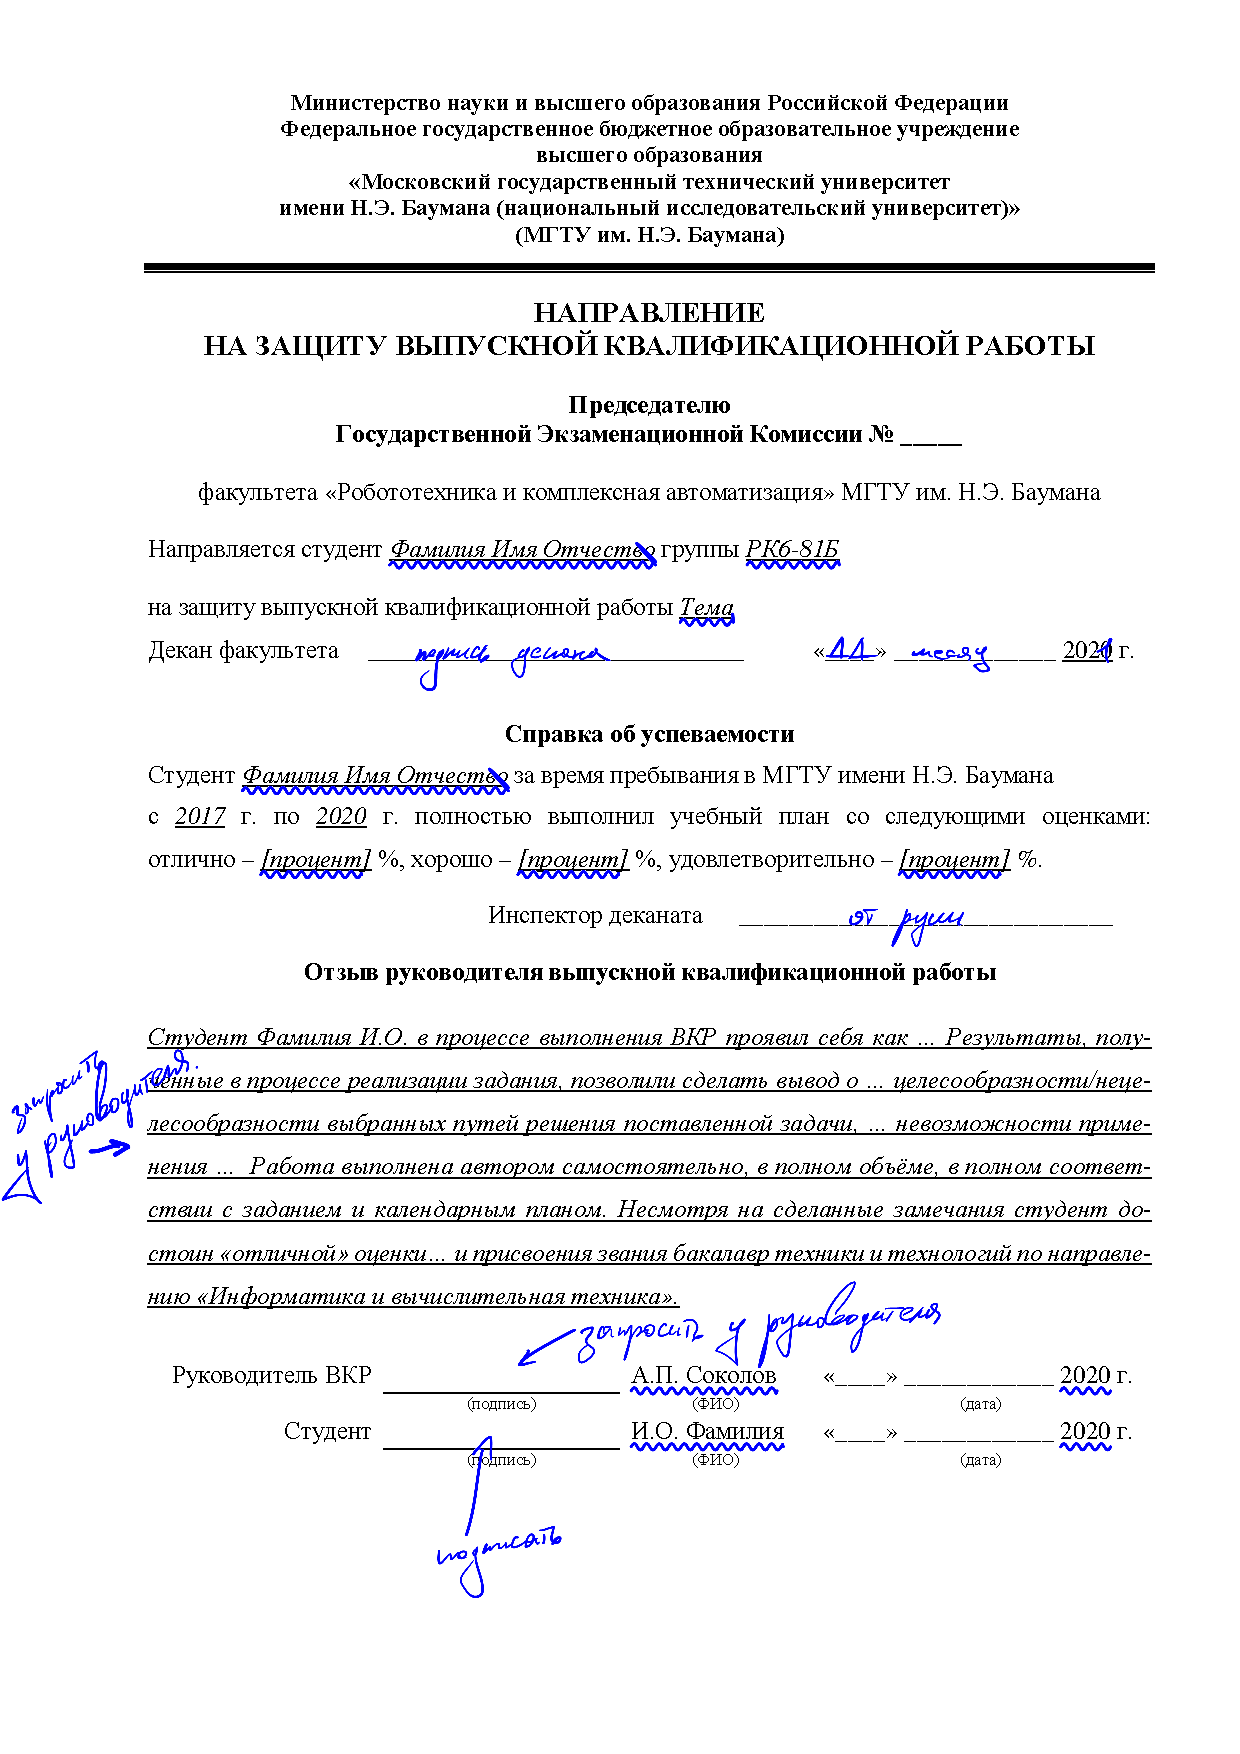
\includepdf{doc-additional/cpxsln_vkr_20YY_ShortTitle_group_SurnameNF_referral_for_defense_signed.pdf}
}
%----------------------------------------------------------------

    }
%----------------------------------------------------------
% Реферат
    %----------------------------------------------------------
\chapter*{РЕФЕРАТ}
%----------------------------------------------------------
\doctype\xspace: \total{page}~с., \total{cchapter}~глав, \total{ffigure}~рис., \total{ttable}~табл., \total{bibcnt}~источн.%, \textbf{apxchapters} прил.

\vspace{3mm}

%Ключевые слова:
% \MakeUppercase{\keywordsru}.

\Preface

\textbf{Тип работы}: \doctype.

\textbf{Тема работы}: \textit{<<\Title>>}.

\textbf{Объект исследования}: \ObjectOfResearch.

% При оформлении согласно ГОСТ 7.32-2001 
%(все освещать следует в этом же порядке - разделы не обязательны)
%объект исследования или разработки
%цель работы
%метод или методологию проведения работы
%результаты работы
%основные конструктивные, технологические и технико-эксплуатационные характеристики
%степень внедрения
%рекомендации по внедрению или итоги внедрения результатов НИР
%область применения
%экономическую эффективновность или значимость
%прогнозные предположения о развитии объекта исследования.


%----------------------------------------------------------
% Сокращения и определения
    \newpage
    \pagestyle{fancy}
    \printglossary[type=\acronymtype, title={СОКРАЩЕНИЯ}, nopostdot=false, nonumberlist]
%\thispagestyle{plain}
%\printglossary[type=main, title={ОПРЕДЕЛЕНИЯ}, nopostdot=true]
%----------------------------------------------------------
% Содержание
% Глубина содержания должна быть не более, чем глава (chapter), раздел (section) и подраздел (subsection) 
    \setcounter{tocdepth}{2}
% Добавление в оглавление сверху Стр.
%\makeatletter
%\addtocontents{toc}{\string\pagestyle{TOC}}
%\addtocontents{toc}{\string\thispagestyle{fancy}}
%\addtocontents{toc}{\hfill Стр.\par}
%\def\ps@TOC{%
    %\def\@oddhead{\hfill \thepage \hfill Стр.} % нечетные хедеры
    %\let\@oddfoot\@empty % нечетные футеры
    %\def\@evenhead{\hfill \thepage \hfill Стр.} % четные хедеры
    %\let\@evenfoot\@empty % четные футеры
%}
%\makeatother
%----------------------------------------------------------
    \renewcommand{\contentsname}{\MakeUppercase{Содержание}}
    \newpage
%\pagestyle{tocpage}
    \tableofcontents
%----------------------------------------------------------
% Введение
    {%
        \def\thesection{В.\arabic{section}}
        \def\thefigure{В.\arabic{figure}}
        \def\thetable{В.\arabic{table}}
        %----------------------------------------------------------
\chapter*{ВВЕДЕНИЕ}\label{chap.introduction}
\addcontentsline{toc}{chapter}{ВВЕДЕНИЕ}
% =========================================================================== %
% ----------------------------- ОСНОВНЫЕ ПУНКТЫ ----------------------------- %
% 1. Описание задач, в которых нужно всякое навороченное математическое ПО
% 2. Примеры наовороченного математического ПО
%   2.1. Почему просто математического ПО не всегда достаточно?
%   2.2. Упомянуть про задачи, у которых одна и та же постановка, но разные 
%         параметры
% 3. Примеры ПО, которое рассчитано на многократное решение задач, автоматизи-
%    рующее их решение (Scientific workflow, hallo?)
%   3.1. Использование графов при описании логики решения в системах научных
%        расчётов
%   3.2. Неудобства в описании данных
%   3.3. Визуальное программирование
% 4. Итог: нужно ПО, где есть какая-то абстракция над обрабатываемыми данными,
%    где они конкретизируются непосредственно в реализациях этапов алгоритма.
% 5. Enter GBSE and comsdk
%    5.1. А чем оно, собсна, так привлекательно?
%    5.2. Сказать про НОВЫХ пользователей (Р А С Ш И Р Я Е М О С Т Ь)
% 6. Сравнение GBSE и DFD
% =========================================================================== %
Современные научно-технические исследования зачастую включают в себя задачи, при решении которых требуется большое количество вычислений, для которых задействуются большие вычислительные мощности. К таким задачам относятся, например, задачи анализа, определения характеристик материалов или технических объектов, моделирования сложных динамических процессов. Как правило, для решения подобных задач применяется или разрабатывается специализированное программное обеспечение (далее -- \glsxtrshort{ПО}).

Среди прочих применяются программные продукты, предоставляющие пользователю формальный язык описания математических выражений и его интерпретатор, выполняющий необходимые вычисления на машине пользователя. К таким системам относятся, например, Mathcad. Также стоит отметить системы специализирующиеся на символьной алгебре, такие, как Maple\cite{CharMaple1983} и Wolfram Mathematica. В настоящее время данные программные комплексы поддерживают решение задач из различных областей математики, включающих в себя теорию графов, теорию множеств и~т.д, предоставляют инструменты визуализации и анализа результатов. Все они позволяют выполнять математическое моделирование, в том числе, сложных технических объектов. При всех их преимуществах необходимость формулировать математические постановки решаемых задач (т.е.~формировать математические модели, составлять системы уравнений и~т.д.) остаётся за пользователем. Зачастую требуется решать множество задач с схожей постановкой, но с различными входными параметрами. Такая необходимость, например, возникает при решении задач оптимизации, где критерием является некоторая характеристика, получаемая в результате решения задачи анализа. Следовательно, целесообразны автоматизированные средства решения типовых задач анализа и моделирования.

Данные средства относятся к специализированному \glsxtrshort{ПО}, а потому при их разработке требуются глубокие познания в предметной области. Кроме того, важно, чтобы создаваемая кодовая база была рассчитана на дальнейшую поддержку, что предъявляет соответствующие требования к структуре исходного кода и документации. Таким образом целесообразно применение некоторых средств, позволяющих организовать разработку программного обеспечения для решения задач моделирования и анализа и повысить его поддерживаемость.

В наши дни популярность приобретает применение т.н. научных систем управления потоком задач (англ.~scientific workflow systems). Они предоставляют средства организации этапов решения вычислительной задачи и управления вычислительными ресурсами. Процесс работы с подобными системами состоит из 4 основных этапов:
\begin{enumerate}[1)]
  \item составление описания операций обработки данных и зависимостей между ними;
  \item распределение процессов обработки данных по вычислительным ресурсам;
  \item выполнение обработки данных;
  \item сбор и анализ результатов и статистики~\cite{DeelmanWorkflow2009}.
\end{enumerate}

Примерами подобных систем могут служить Pegasus\cite{DeelmanPegasus2016}, Kepler\cite{AltintasKepler2004} и pSeven\cite{NazarenkoDFM2015}. Помимо инструментов загрузки пользовательских реализаций этапов решения задачи они, как правило, представляют библиотеку типовых действий и преобразований, таких, как считывание данных и их сохранение в файлы одного из поддерживаемых форматов, операции со строками, работы с базами данных, и~т.д. Кроме того, некоторые из них имеют средства интеграции с другими системами моделирования и анализа, что позволяет задействововать их при расчётах. На рисунке~\ref{fig:intro.keplerScreenshot} изображён пример описания некоторого процесса в системе Kepler.
\begin{figure}[!ht]
  \centering
  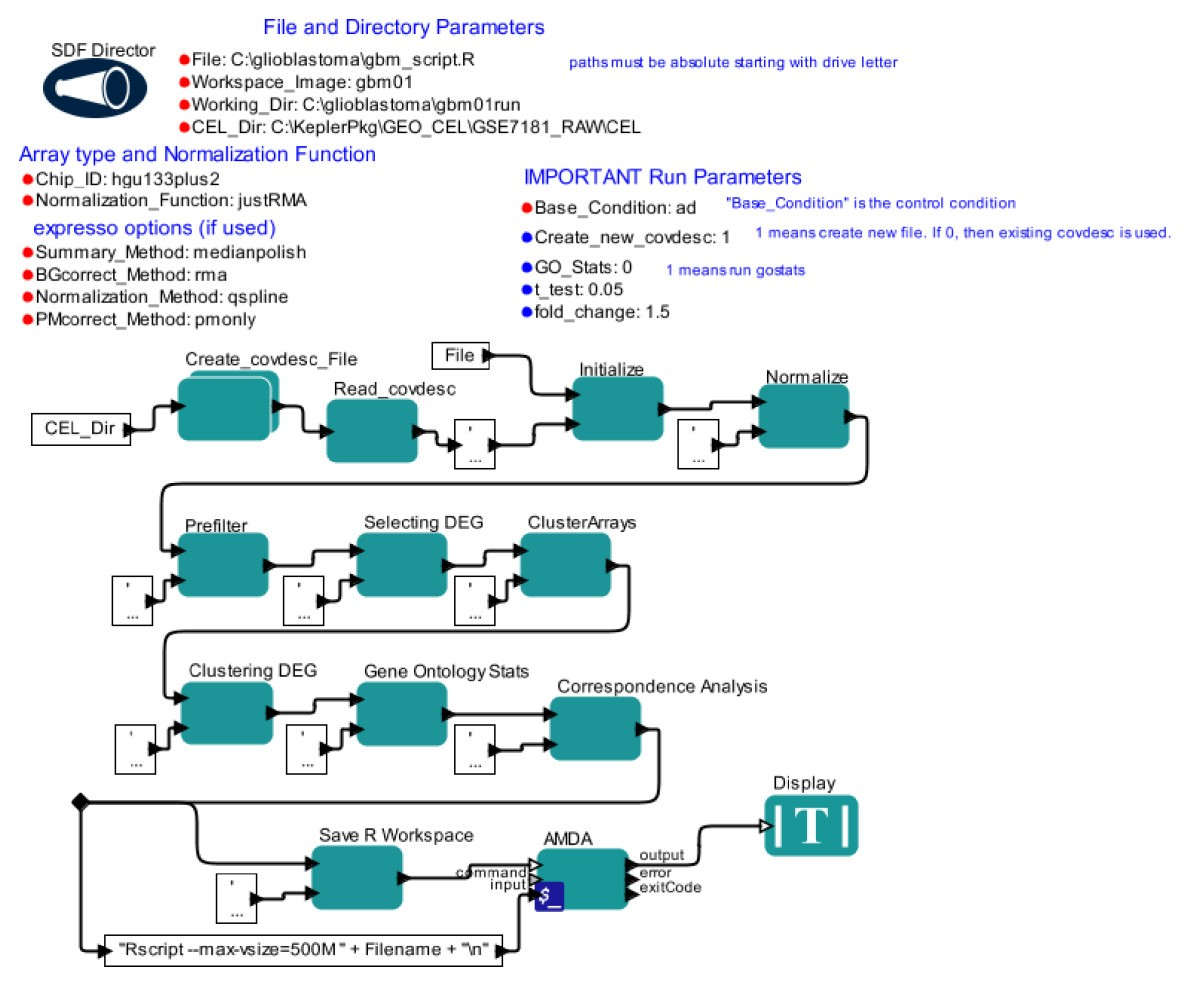
\includegraphics[height=0.35\textheight]{figures/screenshot.KeplerWorkflow.jpg}
  \caption{Описание процесса обработки данных в системе Kepler}
  \label{fig:intro.keplerScreenshot}
\end{figure}

Кроме того, для облегчения процесса разработки трудоёмкого ПО существуют т.н. платформы малокодовой разработки (англ.~low-code development platforms, \glsxtrshort{LCPD})\cite{DiRuscio2022}. В них, подобно системам управления потоком задач, логика разрабатываемого программного продукта описывается при помощи некоторого формального языка или с использованием графического редактора. От системы к системе подход к описаниям варьируется. Может применяться структурный подход, описывающий шаги алгоритма, или предметно-ориентированный, при котором описываются взаимодействующие сущности. Некоторые системы позволяют по созданному описанию генерировать готовые компоненты будущего программного продукта. Так платформа Codebots реализует предметно-ориентированный подход и по составленным UML-диаграммам взаимодействующих сущностей позволяет генерировать \glsxtrshort{API}, \glsxtrshort{JSON}-схемы данных и документацию\cite{DiRuscio2022}. Тем не менее, при реализации сложных вычислительных методов целесообразнее использовать структурный подход.

Одной из ключевых особенностей описанных технологических решений является выделение операций обработки данных в отдельные программные модули (функции, подпрограммы, скрипты). Как правило, при создании описаний алгоритмов в них используется следующий подход. Поскольку известно, что выходные данные одного программного модуля могут являться входными для одного или нескольких других модулей, можно сказать, что между ними формируются зависимости по входным и выходным данным. Тогда возможно составить такой ориентированный граф, описывающий общую логику алгоритма, в котором узлами являются операции обработки данных, а рёбрами -- пути данных. Такой подход получил название ``диаграммы потоков данных'' (англ.~Dataflow Diagram, \glsxtrshort{DFD}). На рисунке~\ref{fig:exampleDataflow} приведён пример такого ориентированного графа, описывающего процесс вычисления среднего арифметического и среднего геометрического двух массивов вещественных чисел.
\begin{figure}
  \centering
  \includegraphics[width=\textwidth]{figures/example.dataflow.png}
  \caption{Пример диаграммы потоков данных}
  \label{fig:exampleDataflow}
\end{figure}

При известных входных и выходных данных каждого модуля они могут создаваться независимо друг от друга\cite{DanilovPar2011}. Возникает возможность распределения задач создания отдельных программных модулей между разработчиками. Таким образом, уменьшается объём работы по написанию исходных кодов, приходящийся на одного исследователя. Это в свою очередь облегчает отладку и написание документации, что положительно сказывается на общем качестве реализуемого ПО.

В приведённом выше подходе существует необходимость явно описывать входные и выходные данные каждого процесса обработки. При этом на начальных этапах проектирования не всегда данные требуемые данные могут быть полность определены в силу недостатка представлений о программной реализации тех или иных этапов. Таким образом, в некоторых случаях может быть целесообразен такой подход к построению описания логики реализуемого решения, что в нём не указываются конкретные обрабатываемые данные. Последовательность выполнения отдельных этапов в таком случае должна задаваться явно. В предпринимательстве и управлении проектами подобный подход широко распространён и реализован в сетевых графиках. Сетевой график представляет собой ориентированный граф, в котором вершины -- это события или состояния проекта, а рёбра -- это работы. В работе~\cite{SokolovPershin2018} рассматривается применение идеи переходов между состояниями при описании логики вычислительных алгоритмов. Описанный подход получил название graph-based software engineering (\glsxtrshort{GBSE}). Кроме того в указанной работе описана реализация GBSE в библиотеке comsdk для языка C++.

Был проведён сравнительный анализ программного каркаса comsdk с аналогичным программным комплексом, в котором реализованы диаграммы потоков данных. В качестве такой реализации был рассмотрен программный комплекс pSeven, разработанный отечественной компанией DATADVANCE. Он направлен в первую очередь на решение конструкторских, оптимизационных задач и, помимо этого, задач анализа данных, что в первом приближении делает его аналогом comsdk по предметному назначению.

В терминах \textsf{pSeven}: графовое описание процесса решения задачи называется \textit{расчетной схемой} (англ.~workflow); вершинам графового описания поставлены в соответствие процессы обработки данных (используется термин \textit{блоки}), а рёбра определяют \textit{связи} между блоками и направления передачи данных между процессами~\cite{NazarenkoDFM2015}. При работе с pSeven используются следующие понятия:
\begin{itemize}
  \item \textsf{расчётная схема} -- формальное описание процесса решения некоторой задачи в виде ориентированного графа;
  \item \textsf{блок} -- программный контейнер для некоторого процесса обработки данных, входные и выходные данные для которого задаются через порты (см.~ниже);
  \item \textsf{порт} -- переменная конкретного\footnote{Динамическая типизация не поддерживается.} типа, определённая в блоке и имеющая уникальное имя в его пределах;
  \item \textsf{связь} -- направленное соединение типа ``один к одному'' между выходным и входным портами разных блоков.
\end{itemize}

С учётом данных понятий можно описать используемую методологию диаграмм потоков данных следующим образом. Расчётная схема содержит в себе набор процессов обработки данных (блоков), каждый из которых имеет (возможно, пустой) набор именованных входов и выходов (портов). Данные передаются через связи. Для избежания т.н. гонок данных (англ.~data races) множественные связи с одним и тем же входным портом не поддерживаются. Для начала выполнения каждому блоку требуются данные на всех входных портах. Все данные на выходных портах формируются по завершении исполнения блока~\cite{NazarenkoDFM2015}.

Сравнение реализаций двух подходов проводилось по следующим критериям:
\begin{itemize}
  \item особенности реализуемого подхода,
  \item особенности программной реализации,
  \item особенности взаимодействия пользователя с реализованной системой.
\end{itemize}
С учётом этого были выделены конкретные признаки для сравнения:
\begin{itemize}
  \item предметное назначение,
  \item значение вершины графа, описывающего алгоритм,
  \item значение ребра графа, описывающего алгоритм,
  \item топология графа, описывающего решение,
  \item поддержка иерархических графовых описаний, когда одно графовое описание является частью (ребром или вершиной) другого
  \item принцип передачи данных между отдельными этапами описываемого алгоритма,
  \item необходимость указывать входные и выходные данные каждого шага алгоритма
  \item язык программной реализации,
  \item файловый формат графовых описаний,
  \item файловая структура проекта реализуемого алгоритма,
  \item поддерживаемые типы данных,
  \item принцип ввода входных данных для алгоритма и его параметров,
  \item принцип вывода результатов работы алгоритма,
  \item поддержка параллельного выполнения незавимых шагов алгоритма,
  \item поддержка распределённого выполнения отдельных этапов алгоритма на вычислительном кластере,
  \item наличие графического редактора графовых описаний
  \item средства визуализации результатов работы алгоритма,
  \item поддержка алгоритмов, требующих принятие решения от пользователя,
  \item возможность дополнения набора входных данных во время работы алгоритма.
\end{itemize}

Результаты проведённого сравнения представлены в таблице \ref{rndhpcblo.0209}.

\begin{landscape}
  \begin{longtable}{|c|p{0.3\textwidth}|p{0.55\textwidth}|p{0.55\textwidth}|}
    \caption{Сравнительная таблица}\label{rndhpcblo.0209}                                                                                                                                                                                                                                                                                                                                                                                                                                                                                                                                                                                                                                                                                                                                                                                                                                                                                                                                                                                                           \\
    \hline
    \textbf{№} & \textbf{Признак}                                                                           & \textbf{pSeven}                                                                                                                                                                                                                                                                                                                                                                                                                                                                                                                                                                                                                                                   & \textbf{comsdk}                                                                                                                                                                                                                                                                   \\
    \hline
    1          & Предметное назначение                                                                      & Задачи оптимизации, анализ данных                                                                                                                                                                                                                                                                                                                                                                                                                                                                                                                                                                                                                                 & Задачи автоматизированного проектирования, алгоритмизация сложных вычислительных методов, анализ данных                                                                                                                                                                           \\
    \hline
    2          & Значение вершины графа, описывающего алгоритм                                              & Блок (процесс обработки данных)                                                                                                                                                                                                                                                                                                                                                                                                                                                                                                                                                                                                                                   & состояние данных                                                                                                                                                                                                                                                                  \\
    \hline
    3          & Значение ребра графа, описывающего алгоритм                                                & Связь (направление передачи данных)                                                                                                                                                                                                                                                                                                                                                                                                                                                                                                                                                                                                                               & переход меду состояниями с указанием функций, осуществляющих переход                                                                                                                                                                                                              \\
    \hline
    4          & Топология графа, описывающего решение                                                      & По умолчанию поддерживаются только ациклические графы. Поддерживаемая топология расширяется засчёт специальных управляющих блоков, которые отслеживают выполнение условий: для условного ветвления используется блок "Условие" (англ. condition), который перенаправляет данные на один из выходных портов в зависимости от выполнения описанного условия (подробнее см. \cite{pSevenDocsConditons2022}); Для реализации циклов в общем случае используются блоки "Цикл" (англ. loop)\cite{pSevenDocsWorkflow2021}, но для некоторых задач существуют специализированные блоки, организующие логику работы цикла (например, блок "Оптимизатор" (англ.~optimizer)) & Любая                                                                                                                                                                                                                                                                             \\
    \hline
    5          & Поддержка иерархических графовых описаний                                                  & \multicolumn{2}{c|}{Присутствует}                                                                                                                                                                                                                                                                                                                                                                                                                                                                                                                                                                                                                                                                                                                                                                                                                                                                                                                     \\
    \hline
    6          & Принцип передачи данных между отдельными этапами описываемого алгоритма                    & Данные между узлами передаются согласно определйнным связям, которые на уровне выполнения создают пространство в памяти для ввода и вывода данных для выполняемых в раздельных процессах блоков. Транзитная передача данных, которые не изменяются в данном блоке, на выход невозможна.                                                                                                                                                                                                                                                                                                                                                                           & Поскольку узлами графа являются состояния данных, существует возможность задействовать в расчётах только часть данных, оставляя их другую часть неизменной. Фактической передачи данных не производится.                                                                          \\
    \hline
    7          & Необходимость указывать входные и выходные данные каждого шага алгоритма                   & Присутствует                                                                                                                                                                                                                                                                                                                                                                                                                                                                                                                                                                                                                                                      & Отсутствует                                                                                                                                                                                                                                                                       \\
    \hline
    8          & Язык программной реализации                                                                & \multicolumn{2}{c|}{С++, Python}                                                                                                                                                                                                                                                                                                                                                                                                                                                                                                                                                                                                                                                                                                                                                                                                                                                                                                                      \\
    \hline
    9          & Файловый формат графовых описаний                                                          & Расчетная схема (в форме орграфа) сохраняется в двоичный файле закрытого формата с расширением \textsf{.p7wf}.                                                                                                                                                                                                                                                                                                                                                                                                                                                                                                                                                    & Графовая модель (определяет алгоритм проведения комплексных вычислений в форме орграфа) сохраняется в текстовом файле открытого формата, подготовленного на языке \gls{aDOT}\cite{SokolovADOT2020}, являющегося ``сужением'' (частным случаем) известного формата DOT (Graphviz). \\
    \hline
    10         & Файловая структура проекта реализуемого алгоритма                                          & Проект состоит из непосредственно файла проекта, в котором хранятся ссылки на созданные расчётные схемы и локальную базу данных, сами расчётные схемы, файлы с их входными данными, файлы отчётов, где сохраняются выходные данные последних расчётов и результаты их анализа.                                                                                                                                                                                                                                                                                                                                                                                    & Проект состоит из \textsf{.aDOT} файла с описанием графа, \textsf{.aINI}-файлов с описанием форматов входных данных, библиотек функций-обработчиков, функций-предикатов и функций-селекторов, файлов, куда записываются выходные данные.                                          \\
    \hline
    11         & Поддерживаемые типы данных                                                                 & Целые числа, числа с плавающей точкой, строки, логические переменные, логические, целочисленные и вещественные векторы и матрицы                                                                                                                                                                                                                                                                                                                                                                                                                                                                                                                                  & Целые и вещественные числа, строки, целочисленные и вещественные векторы                                                                                                                                                                                                          \\
    \hline
    12         & Принцип ввода входных данных для алгоритма и его параметров                                & Входные данные должны быть указаны при настройках внешних входных портов расчётной схемы.                                                                                                                                                                                                                                                                                                                                                                                                                                                                                                                                                                         & Входные данные хранятся в файле в формате \gls{aINI}\cite{SokAINI}, откуда считываются при запуске обхода графа~\cite{SokolovPershin2017}.                                                                                                                                        \\
    \hline
    13         & Принцип вывода результатов работы алгоритма                                                & Данные с выходных портов схемы сохраняются в локальной базе данных. Для их записи в файлы для обработки/анализа вне pSeven необходимо воспользоваться специально предназначенными для этого блоками.                                                                                                                                                                                                                                                                                                                                                                                                                                                              & Для записи выходных/промежуточных данных в файлы или базы данных необходимо добавить соответствующие функции-обработчики. Формат выходных данных не регламентирован.                                                                                                              \\
    \hline
    14         & Поддержка параллельного выполнения независимых шагов алгоритма                             & Присутствует. Блоки, входящие в состав различных ветвлений схемы могут быть выполнены параллельно, поскольку они не зависят друг от друга по используемым данным.                                                                                                                                                                                                                                                                                                                                                                                                                                                                                                 & Присутствует. Существует возможность обойти различные ветвления графа одновременно.                                                                                                                                                                                               \\
    \hline
    15         & Поддержка распределённого выполнения отдельных этапов алгоритма на вычислительном кластере & Присутствует                                                                                                                                                                                                                                                                                                                                                                                                                                                                                                                                                                                                                                                      & В текущей версии отсутствует                                                                                                                                                                                                                                                      \\
    \hline
    16         & Наличие графического редактора графовых описаний                                           & Да                                                                                                                                                                                                                                                                                                                                                                                                                                                                                                                                                                                                                                                                & Да\footnote{В виде отдельного веб-приложения}                                                                                                                                                                                                                                     \\
    \hline
    17         & Средства визуализации результатов работы алгоритма                                         & Реализованы как часть системы формирования отчётов (см. выше)                                                                                                                                                                                                                                                                                                                                                                                                                                                                                                                                                                                                     & В текущей версии отсутствуют                                                                                                                                                                                                                                                      \\
    \hline
    18         & Поддержка алгоритмов, требующих принятие решения от пользователя                           & По умолчанию отсутвует. Требуется реализация дополнительных скриптов на языке Python, отвечающих за взаимодействие с пользователем                                                                                                                                                                                                                                                                                                                                                                                                                                                                                                                                & Частично присутствует засчёт средства генерации форм ввода\cite{SokolovPershin2017}                                                                                                                                                                                               \\
    \hline
    19         & Возможность дополнения набора входных данных во время работы алгоритма                     & Отсутствует                                                                                                                                                                                                                                                                                                                                                                                                                                                                                                                                                                                                                                                       & Частично реализована при помощи функций-обработчиков специального типа, создающих формы ввода                                                                                                                                                                                     \\
    \hline
  \end{longtable}
\end{landscape}

Таким образом, на данный момент comsdk обладает сравнительно меньшим числом функциональных возможностей, чем современные научные системы управления потоком задач, подобные pSeven, но предоставляет потенциально больше средств для взаимодействия реализуемых алгоритмов с пользователем. В условиях существующей на сегодняшней день потребности в отечественном программном обеспечении для реализации сложных численных методов, актуально развитие данного программного каркаса.
    }
%----------------------------------------------------------
    \mainmatter %% это включает нумерацию глав и секций в документе ниже
%----------------------------------------------------------
    %=============================================================
% ---------------------------------------------------
\chapter{Обзор средств взаимодействия пользователя в графоориентированных системах} \label{chap1.comparison}
Среди вычислительных задач, с которыми сталкиваются современные исследователи и разработчики наукоёмкого программного обеспечения, можно выделить те, в которых в результате проведения расчётов получается несколько различных результатов, из которых требуется выбрать наиболее подходящий на основе каких-то критериев или провести ту или иную операцию в зависимости от полученных результатов. В наши дни наблюдается тенденция к автоматизации подобного процесса на основе различных алгоритмов анализа и принятия решений, некоторые из которых разрабатываются специально под конкретную задачу, а некоторые, более универсальные, адаптируются под неё, как, например, описано в \cite{KatalOpt2020}. Тем не менее, остаётся широкий спектр задач, где разработка подобных алгоритмов не ведётся ввиду слишком узкой направленности или отсутствии технической возможности автоматизировать принятие решений (как правило, в исследовательских задачах). В таких случаях за него отвечает лицо, принимающее решение (\glsxtrshort{ЛПР}). При разработке универсального программного комплекса, позволяющего решать различные задачи проектирования и оптимизации было бы полезно включить возможность \glsxtrshort{ЛПР} взаимодействовать с промежуточными результатами вычислений. Помимо прочего, подобная необходимость возникает, когда:
\begin{enumerate}
    \item нет формально определённых критериев отбора, на основе которых его можно было бы автоматизировать;
    \item критериев анализа результатов слишком много для того, чтобы реализовать автоматизированную процедуру для его проведения в пределах исследовательской работы;
\end{enumerate}

Поскольку в данной работе рассматривается, в первую очередь, система, реализующая графоориентированный подход к решению сложных вычислительных задач, то целесообразно рассмотреть подходы к организации взаимодействия пользователя с процессом решения. На основании изложенного выше были выделены следующие сценарии взаимодействия с пользователем в данной системе:
\begin{itemize}
    \item Введение дополнительных данных, которые требуются на дальнейших этапах расчётов, но которые не были получены автоматически до этого;
    \item Выбор конкретных данных из некоторого однородного набора для его сужения;
    \item Выбор дальнейшей логики выполнения расчётов на основании полученных на текущем этапе результатов.
\end{itemize}
Помимо этого, для эффективной работы с подобной системой исследователю необходим графический пользовательский интерфейс, в котором модель организации вычислений может быть представлена визуально. Большие перспективы в автоматизации процесса решения сложных задач перед исследователем открывает возможность прямого взаимодействия с вычислительной моделью: остановка вычислительного процесса на определенном этапе, изучение обрабатываемых данных, просмотр истории изменения обрабатываемых данных, возврат к определенному этапу вычислений, ввод
дополнительных параметров на определенной
стадии вычислений и т. д.\cite{SokolovCADCMInteraction2021}
Кроме того, целесообразно рассмотреть основные понятия, вводимые в данной системе.
\begin{itemize}
    \item \emph{Состояние данных} - некоторый набор данных, в котором они хранятся тройками вида "тип - имя - значение". В GBSE реализован в виде специального класса с названием \textsf{Anymap}.
    \item \emph{Функция-обработчик} - функция, которая вызывается при переходе из одного состояния данных в другое. Фактически данная функция каким-то образом модифицирует объект состояния данных.
    \item \emph{Функция-предикат} - функция, связанная с тем же переходом, что и некоторая функция-обработчик, проверяющая соответствие входных данных тому формату, в котором они ожидаются на входе обработчика.
\end{itemize}
На концептуальном уровне абстракции в рассматриваемой системе получение каких-то данных или решений от пользователя может быть реализовано, как и любой другой процесс модификации данных, через соответствующие функции-обработчики и предикаты. Рассмотрим возможные подходы к реализации сценариев взаимодействия пользователя, описанных выше.

Для введения дополнительных данных в GBSE реализован специальный инструмент автоматической генерации графических программных интерфейсов (\glsxtrshort{GUIen}) с формами ввода необходимых данных\cite{SokolovPershin2017}, однако этот инструмент ещё не связан с основным графоориентированным программным каркасом. Средства, реализующие два других сценария на момент написания данной работы находятся в разработке. Для предоставления пользователю возможности сделать выбор относительно дальнейшей обработки данных необходимо разработать следующие средства:
\begin{enumerate}
    \item Средство визуализации текущего состояния данных
    \item Средство содержательной интерпретации текущего состояния данных
\end{enumerate}
Кроме того, для реализации рассматриваемых сценариев будет необходимо доработать средство генерации форм ввода и реализовать в нём дополнительную категорию форм, направленных не на внесение новых данных, а на выбор, в том числе и множественный, из представленных вариантов, отображённых, в том числе, и с помощью средства визуализации.
%----------------------------------------------------------
%----------------------------------------------------------
\chapter{Сравнительная характеристика программных комплексов, реализующих графоориентированный подход}
%----------------------------------------------------------
Помимо обзора потенциальных сценариев взаимодействия пользователя с системой в процессе обхода графовой модели была проведена сравнительная характеристика рассматриваемой разработки с представленными в настоящее время на рынке продуктами.
В рамках сравнения были рассмотрены известные программные комплексы, в основе которых в том или ином виде лежит идея организации вычислений, описываемая с помощью ориентированных графов (графоориентированный подход).

Для проведения сравнения с программным каркасом GBSE выбирались программные продукты, в которых так или иначе реализован описанный выше подход. В первую очередь был рассмотрен программный комплекс pSeven, разработанный отечественной компанией DATADVANCE. Он направлен в первую очередь на решение конструкторских, оптимизационных задач и, помимо этого, задач анализа данных, что в первом приближении делает его аналогом GBSE по предметному назначению. У автора работы присутствует опыт работы с этим комплексом в рамках прохождения курса лабораторных работ по изученной на кафедре дисциплине "Методы оптимизации". В данном курсе были освещены основы работы с pSeven и основные приниципы организации вычислений в нём. Таким образом, на момент выбора программных комплексов для сравнения уже имелась некоторая информация о pSeven, которая позволила включить его в рассмотрение.

Кроме того, научным руководителем данной работы была рекомендована разработка отечественной компании ``Ладуга'' PRADIS - комплекс, так же направленный на решение конструкторских задач. В данной разработке основной упор сделан на задачи анализа проектных решений на микро- и макроуровне.

\section{Выделение признаков для сравнения}

% При выделении сравнительных признаков необходимо было, чтобы они охватывали достаточно широкую область сведений о программном продукте.

Среди прочих должны были быть выделены признаки, относящиеся как к общей структуре программного комплекса, так и к особенностям реализации в нём графоориентированного подхода и, кроме того, к особенностям взаимодействия с пользователем при решении задач, требующих действий с его стороны.

Сравнение осуществлялось с учётом следующих характерных признаков:
\begin{enumerate}
    \item предметное назначение;
    \item принципы формирования графовых моделей;
    \item формат описания графовых моделей;
    \item файловая структура проекта проведения анализа \gls{TO};
    \item особенности работы с входными и выходными данными графовых моделей;
    \item особенности передачи данных между узлами графовых моделей;
    \item поддержка ветвлений и циклов в топологии графовых моделей;
    \item поддержка параллельной обработки данных;
    \item возможность выбрать из набора однотипных промежуточных результатов расчётов некоторые экземпляры и продолжить расчёт только для них;
    \item возможность доопределять входные данные непосредственно во время обхода графовой модели.
\end{enumerate}

\section{Описание сравниваемых комплексов}
\subsection{Программный комплекс Pradis}

Программный комплекс \textsf{Pradis}, разработанный отечественной компанией <<Ладуга>>, предназначен для анализа динамических процессов в системах разной физической природы (механических, гидравлических и т.д.). Как правило, при помощи данного комплекса решаются нестационарные нелинейные задачи, в которых характеристики системы зависят от времени и пространственных координат. Круг задач, которые могут быть решены с помощью \textsf{Pradis}, достаточно широк: возможен анализ любых технических объектов, модели поведения которых представимы системами обыкновенных дифференциальных уравнений (СОДУ). Анализ статических задач обеспечивается как частный случай динамического расчета.

Практические возможности по решению конкретных задач определяются текущим составом библиотек комплекса, прежде всего библиотек моделей элементов~\cite{PradisGeneral2007}. Данный копмплекс был рекомедован к обзору и сравнению, однако, после проведённого обзора официальной документации~\cite{PradisMethods2007} не было получено достаточного представления об использовании элементов графоориентированных подходов в данном копмлексе, поэтому было принято решение исключить его из дальнейшего рассмотрения.

\subsection{Программный комплекс pSeven}

В программном комплексе \textsf{pSeven}, разработанном компанией DATADVANCE, используется методология диаграмм потоков данных (англ.~Dataflow diagram, DFD). В комплексе применяются ориентированные графы (орграфы) для описания процесса решения некоторой задачи проектирования технического объекта. В терминах \textsf{pSeven}: графовое описание процесса решения задачи называется \textit{расчетной схемой} (англ.~workflow), что, помимо прочего, соответствует классическому термину из области математического моделирования; узлам орграфа поставлены в соответствие процессы обработки данных (используется термин \textit{блоки}), а рёбра определяют \textit{связи} между блоками и направления передачи данных между процессами \cite{Nazarenko2015}. 

%...., определяется только зависимостями между входными и выходными данными каждого отдельного процесса их обработки, входящиего в решение . 
Используются следующие базовые понятия \textsf{pSeven}:
\begin{itemize}
    \item \textsf{расчётная схема} -- формальное описание процесса решения некоторой задачи в виде орграфа;
    \item \textsf{блок} -- программный контейнер для некоторого процесса обработки данных, входные и выходные данные для которого задаются через порты (см. ниже);
    \item \textsf{порт} -- переменная конкретного\footnote{Динамическая типизация не поддерживается.} типа, определённая в блоке и имеющая уникальное имя в его пределах;
    \item \textsf{связь} -- направленное соединение типа ``один к одному'' между выходным и входным портами разных блоков.
\end{itemize}

С учётом данных понятий можно описать используемую методологию диаграмм потов данных следующим образом. Расчётная схема содержит в себе набор процессов обработки данных (блоков), каждый из которых имеет (возможно, пустой) набор именованных входов и выходов (портов). Данные передаются через связи. Для избежания т.н. гонок данных (англ. data races) множественные связи с одним и тем же входным портом не поддерживаются. Для начала выполнения каждому блоку требуются данные на всех входных портах. Все данные на выходных портах формируются по завершении исполнения блока \cite{Nazarenko2015}.

\begin{figure}[h]
    \centering
    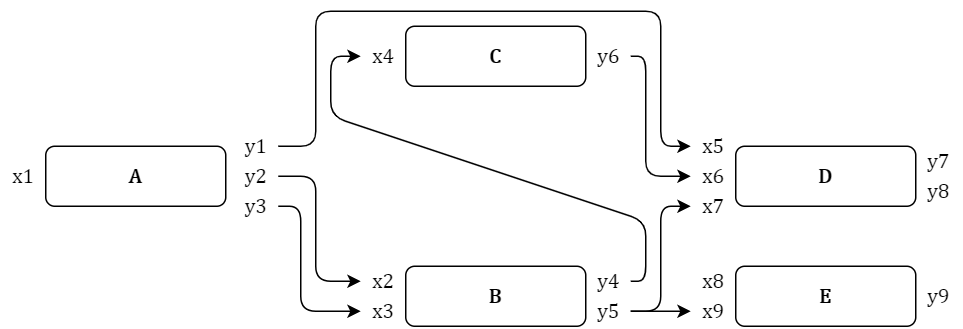
\includegraphics[width=\textwidth]{figures/dataflow.png}
    \caption{Пример диаграммы потоков данных}
    \label{fig:dataflow}
\end{figure}

На рисунке \ref{fig:dataflow} $A, B, C, D$ - блоки обработки информации, $x_i$ - входные порты, $y_i$ - выходные. Стрелками показаны связи. Согласно изложенному выше принципу, сначала будет запущен блок $A$, по его завершении - блок $B$. Затем - блоки $C$ и $E$ (параллельно). По завершении блока $C$ будет запущен блок $D$. На этом обход расчётной схемы завершится, и значения $y_7, y_8$ и $y_9$ будут сохранены в локальной базе данных.

\begin{remark}[принцип обхода в pSeven]
Все порты, которые не привязаны к другим блокам, автоматически становятся внешними входами и выходами для всей расчётной схемы. Для начала обхода расчётной схемы должен быть предоставлен набор входных данных и указаны внешние выходные порты, значения которых обязательно должны быть вычислены в результате обхода. Обход производится в несколько этапов: сперва отслеживаются пути от необязательных выходных портов к входным, все встреченные на пути блоки помечаются, как неактуальные и не будут выполнены в дальнейшем; затем отслеживаются пути от обязательных выходных портов к входным и все встреченные на пути блоки помечаются, как обязательные к исполнению. Наконец, обязательные к исполнению блоки запускаются, начиная с тех, которые подключены к внешним входам расчётной схемы, а неактуальные игнорируются. Обход прекращается, когда не остаётся необходимых для выполнения блоков \cite{Nazarenko2015}. 
\end{remark}

По завершении обхода расчётной схемы результаты расчётов сохраняются в локальной базе данных проекта. В pSeven встроен инструментарий для визуализации и анализа результатов. Схемы, графики, гистограммы и результаты анализа сохраняются в т.н. отчётах - специальных файлах, сохраняемых в директории проекта.

\section{Сравнительная таблица}
Результаты проведённого сравнения представлены в таблице \ref{rndhpcblo.0209}.

\begin{landscape}
\begin{longtable}{|p{0.025\textwidth}|p{0.2\textwidth}|p{0.5\textwidth}|p{0.5\textwidth}|}
    \caption{Сравнительная таблица}\label{rndhpcblo.0209} \\
    \hline
    \textbf{№} & \textbf{Признак} & \textbf{pSeven} & \textbf{GBSE} \\
    \hline
    1 & Предметное назначение & Задачи оптимизации, анализ данных & Задачи автоматизированного проектирования, алгоритмизация сложных вычислительных методов, анализ данных \\
    \hline
    2 & Принцип формирования графовых моделей & Узлы -- блоки (процессы), рёбра -- связи (направление передачи данных) \cite{Nazarenko2015}. & Узлы -- состояния данных, рёбра -- переходы между состояниями, с указанием функций перехода \cite{SokolovPershin2018}. \\
    \hline
    3 & Формат описания орграфа & Расчетная схема (в форме орграфа) сохраняется в двоичный файле закрытого формата с расширением \textsf{.p7wf}. & Графовая модель (определяет алгоритм проведения комплексных вычислений в форме орграфа) сохраняется в текстовом файле открытого формата, подготовленного на языке \gls{aDOT}\cite{SokolovADOT2020}, являющегося ``сужением'' (частным случаем) известного формата DOT (Graphviz). \\
    \hline
    4 & Файловая структура проекта проведения анализа \gls{TO} & Проект состоит из непосредственно файла проекта, в котором хранятся ссылки на созданные расчётные схемы и локальную базу данных, сами расчётные схемы, файлы с их входными данными, файлы отчётов, где сохраняются выходные данные последних расчётов и результаты их анализа. & Проект состоит из \textsf{.aDOT} файла с описанием графа, \textsf{.aINI}-файлов с описанием форматов входных данных, библиотек функций-обработчиков, функций-предикатов и функций-селекторов , файлов, куда записываются выходные данные. \\
    \hline
    5 & особенности работы с входными и выходными данными графовых моделей & Входные данные должны быть указаны при настройках внешних входных портов расчётной схемы. Данные с выходных портов схемы сохраняются в локальной базе данных. Для их записи в файлы для обработки/анализа вне pSeven необходимо воспользоваться специально предназначенными для этого блоками. & Входные данные хранятся в файле в формате \gls{aINI}\cite{SokAINI}, откуда считываются при запуске обхода графа~\cite{SokolovPershin2017}. Для записи выходных/промежуточных данных в файлы или базы данных необходимо добавить соответствующие функции-обработчики. Формат выходных данных не регламентирован. \\
    \hline
    6 & Особенности передачи параметров между узлами графовых моделей & Данные между узлами передаются согласно определйнным связям, которые на уровне выполнения создают пространство в памяти для ввода и вывода данных для выполняемых в раздельных процессах блоков. Транзитная передача данных, которые не изменяются в данном блоке, на выход невозможна. & Поскольку узлами графа являются состояния данных, существует возможность задействовать в расчётах только часть данных, оставляя их другую часть неизменной. \\
    \hline
    7 & Поддержка ветвлений и циклов & Присутствует. Достигается засчёт специальных управляющих блоков, которые отслеживают выполнение условий: для ветвления используется блок "Условие" (англ. condition), который перенаправляет данные на один из выходных портов в зависимости от выполнения описанного условия (подробнее см. \cite{pSevenDocsConditons2022}); Для реализации циклов в общем случае используются блоки "Цикл" (англ. loop)\cite{pSevenDocsWorkflow2021}, но для некоторых задач существуют специализированные блоки, организующие логику работы цикла (например, блок "Оптимизатор" (англ. optimizer)) & Присутствует по умолчанию \\
    \hline
    8 & Поддержка параллельной обработки данных & Присутствует. Блоки, входящие в состав различных ветвлений схемы могут быть выполнены параллельно, поскольку они не зависят друг от друга по используемым данным. & Присутствует. Существует возможность обойти различные ветвления графа одновременно.\\
    \hline
    9 & Возможность выбрать из набора однотипных промежуточных результатов расчётов некоторые экземпляры и продолжить расчёт только для них; & Производится на этапе анализа результатов с помощью отчётов, где можно задать фильтрацию выходных данных согласно указанным критерия. В случае, если результаты являются промежуточными, расчётную схему приходится разбивать на части. & Планируется реализовать средство визуализации данных, которое в совокупности с автоматической генерацией форм ввода\cite{SokolovPershin2017} позволят отбирать корректные результаты промежуточных вычислений во время обхода графовой модели. \\
    \hline
    10 & Возможность доопределения значений входных данных в процессе обхода графа & Отсутствует & Частично реализована при помощи функций-обработчиков специального типа, создающих формы ввода \\
    \hline
\end{longtable}
\end{landscape}
%----------------------------------------------------------


%----------------------------------------------------------
%----------------------------------------------------------
%----------------------------------------------------------
%----------------------------------------------------------
%=============================================================

%----------------------------------------------------------
    \backmatter %% Здесь заканчивается нумерованная часть документа и начинаются Заключение и Список использованных источников
%----------------------------------------------------------
    %----------------------------------------------------------
\chapter*{ЗАКЛЮЧЕНИЕ}\label{chap_conclusion}
\addcontentsline{toc}{chapter}{ЗАКЛЮЧЕНИЕ}
%----------------------------------------------------------

В результате проведенной работы был реализован редактор графов, который является достаточно полезным инструментом, дополняющим предложенный А.П.Соколовым и А.Ю.Першиными графоориетированный программный каркас для реализации сложных вычислительных методов. Редактор позволяет создавать ориентированный граф с нуля, а затем экспортировать созданный граф в формате aDOT, также есть возможность загрузить граф из формата aDOT. С помощью редактора можно получить графовую модель вычислительно метода до его реализации, что позволяет заранее распределить задачи между разработчиками, а также, возможно, увидеть тонкие места в реализуемом методе и уделить им особое внимание. 

%----------------------------------------------------------

%----------------------------------------------------------
% Список литературы
    \bibliographystyle{utf8gost705u}
    \addcontentsline{toc}{chapter}{Литература}
    \bibliography{bibliography}
%----------------------------------------------------------
    \subsubsection*{Выходные данные}
%----------------------------------------------------------
    \textit{\DocOutReference}
%----------------------------------------------------------
% Атрибуты задачи
    \docattributes{}{}{}{}{студент группы \group, \Author}{\Year, \Semestr}
%----------------------------------------------------------
% Акт об отсутствии заимствования (включается только для ВКР, для НИРС и КП не нужно)
% Вставится только при сборке ВКР
    \myconditionaltext{\doctypesid}{vkr}{%
        %----------------------------------------------------------------
% В этот документ следует вставить акт об отсутствии заимствования
% Для КП, НИРС этот документ не включается.
% Предварительно документ следует подготовить в MS Word, подписать, преобразовать в PDF и далее разместить в нужном каталоге
\newpage
{\catcode`\_=11
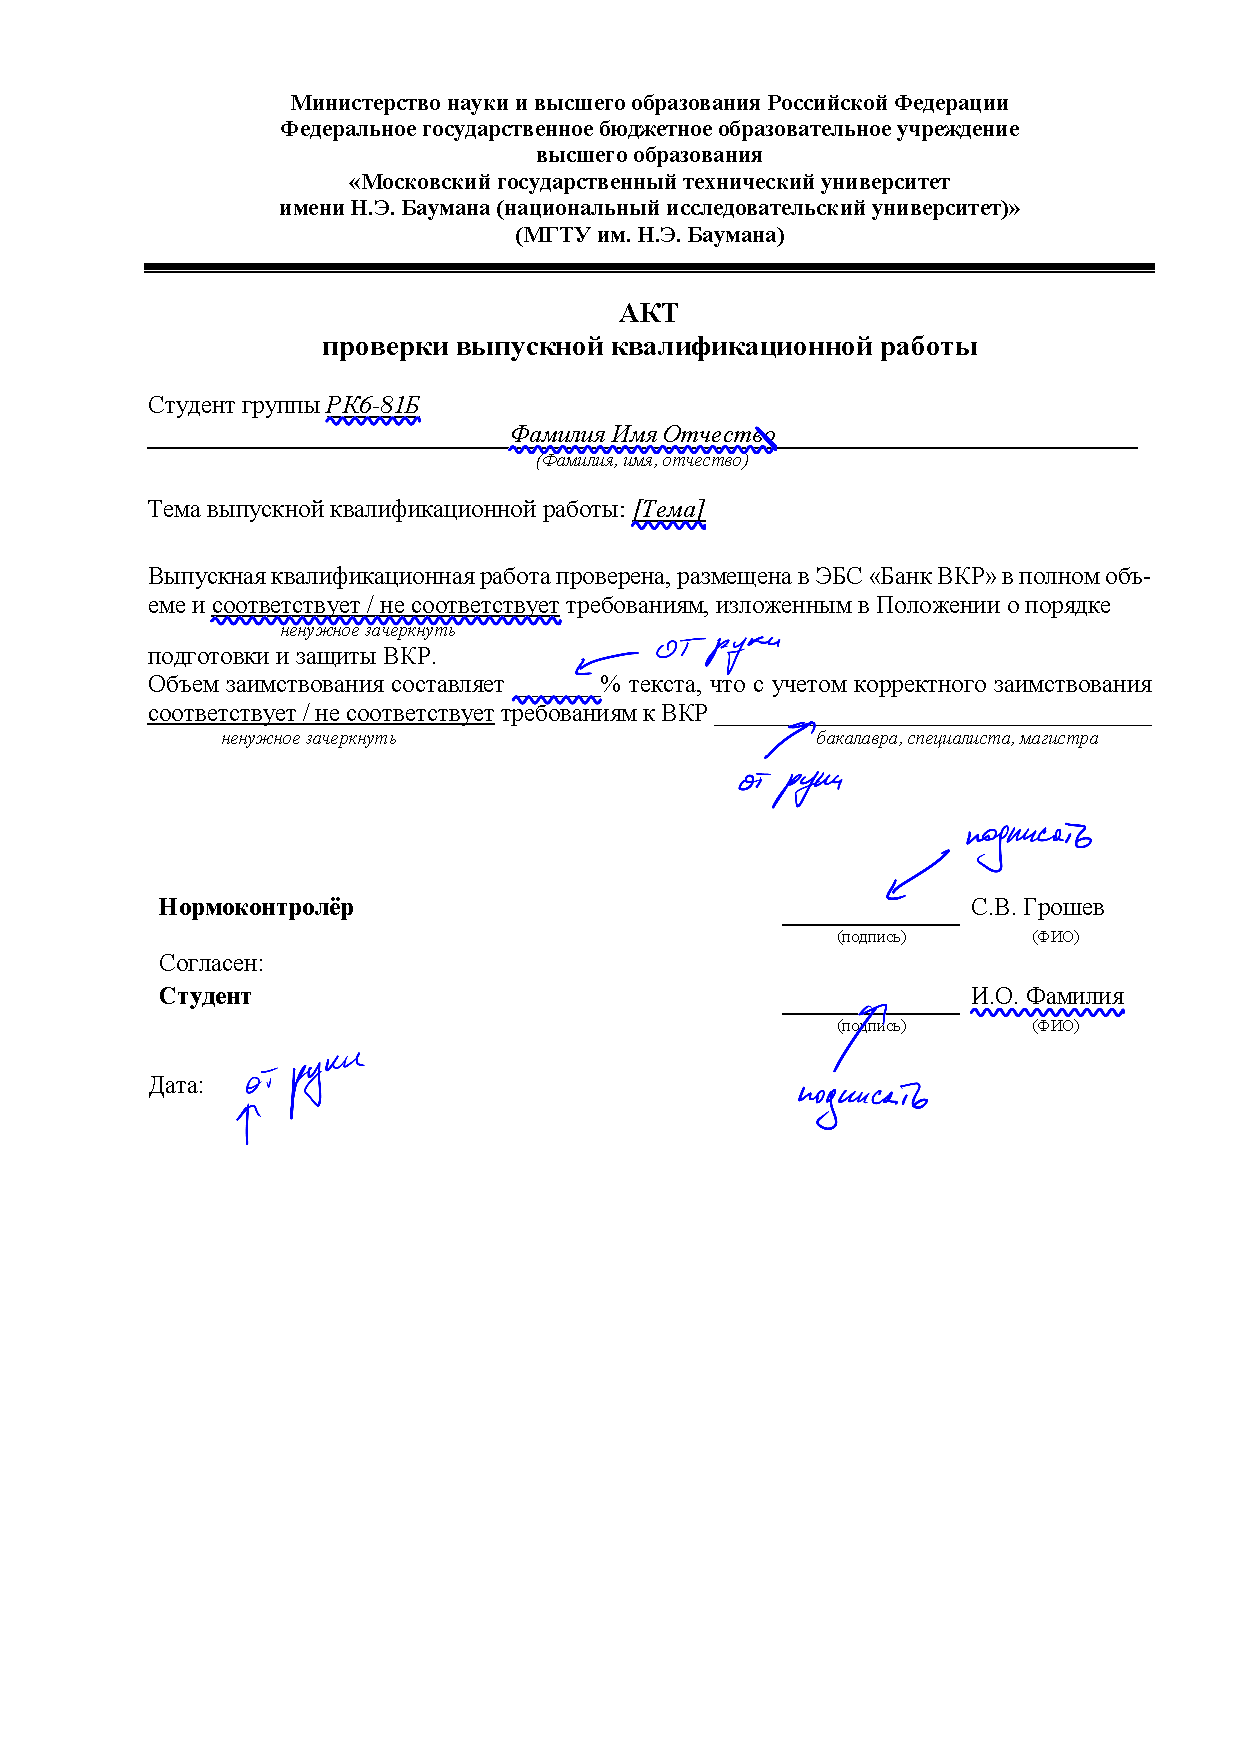
\includepdf{doc-additional/cpxsln_vkr_20YY_ShortTitle_group_SurnameNF_plagiarism.pdf}
}
%----------------------------------------------------------------

    }
%----------------------------------------------------------
    %приложения
%
% листы A1
% Акт об отсутствии заимствований
% Рецензии
%

\appendix

% команды далее необходимы для того, чтобы нумерация элементов текста в приложениях была корректной.
\renewcommand{\theequation}{\thechapter.\arabic{equation}}
\renewcommand{\thefigure}{\thechapter.\arabic{figure}}
\renewcommand{\thetable}{\thechapter.\arabic{table}}
% -------
\renewcommand{\appendixname}{ПРИЛОЖЕНИЯ}
\def\chaptername{ПРИЛОЖЕНИЕ}
\def\thechapter{\Asbuk{chapter}\unskip}
\renewcommand{\thesection}{\thechapter.\arabic{section}\unskip}
%%%%%%%%%%%%%%%%%%%%%%%%%%%%%%%%%%%%%%%%%%%%%%%%%%%%%%%%%%%%%%%%%%%%%%%%
\addcontentsline{toc}{chapter}{ПРИЛОЖЕНИЯ}
%%%%%%%%%%%%%%%%%%%%%%%%%%%%%%%%%%%%%%%%%%%%%%%%%%%%%%%%%%%%%%%%%%%%%%%%
% ПРИЛОЖЕНИЕ
\fancyhead[C]{\thepage \\ \textbf{\leftmark}}
\fancyfoot[C]{}
%----------------------------------------------------------------
\includepdfset{turn=true,scale=0.85,linktodoc=true,pages=-,pagecommand={\pagestyle{fancy}}}
%----------------------------------------------------------------
\chapter{}\label{apx_a1}




%{\catcode`\_=11
%\newpage
%\includepdf[pagecommand=\label{appx_A1_list1},pages=-]{appendices/appx_A1_list1.pdf}
%}
%
%%{\catcode`\_=11
%%\newpage
%%\includepdf[pagecommand=\label{appx_A1_list1},pages=-]{appendices/appx_A1_list1.pdf}
%%}
%%----------------------------------------------------------------
%\chapter{Акты и рецензии}\label{apx_acts_reviews}
%
%{\catcode`\_=11
%\newpage
%\includepdf[pagecommand=\label{appx_act_plagiat},pages=-]{appendices/appx_act_plagiatpdf}
%}
%
%{\catcode`\_=11
%\newpage
%\includepdf[pagecommand=\label{appx_review_1},pages=-]{appendices/appx_review_1.pdf}
%}

%%%%%%%%%%%%%%%%%%%%%%%%%%%%%%%%%%%%%%%%%%%%%%%%%%%%%%%%%%%%%%%%%%%%%%%%




%----------------------------------------------------------
% метка нужна для отслеживания общего числа страниц в документе
    \label{lastpage}
%----------------------------------------------------------
\end{document}
%==========================================================


